\documentclass{xmgr}
\usepackage{graphicx}
\graphicspath{ {images/} }
% Jeśli nowe rozdziały mają się zaczynać na stronach
% nieparzystych:
%\documentclass[openright]{xmgr}

%\defaultfontfeatures{Scale=MatchLowercase}
%\setmainfont[Numbers=OldStyle,Ligatures=TeX]{Minion Pro}
%\setsansfont[Numbers=OldStyle,Ligatures=TeX]{Myriad Pro}
% for fontspec version < 2.0
\setmainfont[Numbers=OldStyle,Mapping=tex-text]{Arial}
\setsansfont[Numbers=OldStyle,Mapping=tex-text]{Arial}
%\setmonofont[Scale=0.75]{Monaco}

% Opcjonalnie identyfikator dokumentu
% drukowany tylko z włączoną opcją 'brudnopis':
\wersja   {wersja wstępna [\ymdtoday]}

\author   {Michał Lipiński}
\nralbumu {105229}
\email    {michal@twoj.cloud}

\author   {Mariusz Piątek}
\nralbumu {205176}
\email    {mariusz.piatek92@gmail.com}

\author   {Paweł Ponieważ}
\nralbumu {228254}
\email    {p.poniewaz@o2.pl}

\title    {Dom Przyszłości w kontekście Internetu rzeczy}
\date     {2016}
\miejsce  {Gdańsk}

\opiekun  {dr Włodzimierz Bzyl}

% dodatkowe polecenia
%\renewcommand{\filename}[1]{\texttt{#1}}
%\definecolor{stress}{cmyk}{0,1,0.13,0} % RubineRed
%\definecolor{topic}{cmyk}{0.98,0.13,0,0.43} % MidnightBlue

\begin{document}

% streszczenie
\begin{abstract}
	Celem niniejszej pracy było udowodnienie, że idea Inteligentnego Domu już dawno przestała być czymś zarezerwowanym dla najbogatszych a~stała się czymś dużo bardziej przystępnym. Niewielkim lub czasem nawet zerowym kosztem można zaimplementować w~swoim domu rozwiązania, które w~znacznym stopniu ułatwią funkcjonowanie mieszkańcom. 
	W~ramach niniejszej pracy stworzono kilka komponentów, które w~połączeniu tworzą solidną podstawę pod zbudowanie Inteligentnego Domu.
	
	Pierwszym komponentem naszego „Inteligentnego Domu na każdą kieszeń” jest system monitoringu. Udało nam się przy pomocy 2 starych telefonów z~aparatem oraz laptopa stworzyć system nadzoru domowego. Przy pomocy framework'a \emph{Meteor} oraz modułu \emph{node-cam}, zabezpieczając wszystko modułem \emph{basic-auth} osiągnęliśmy zerowym kosztem system porównywalny z dostępnymi na rynku komercyjnymi rozwiązaniami.
	
	Następnie, również niewielkim kosztem, stworzyliśmy system inteligentnych świateł. Zamówione z~serwisu \emph{AliExpress} sterowniki, kierowane za pomocą aplikacji \emph{Magic Home}, umożliwiły sterowanie oświetleniem w~sposób nieosiągalny dla tradycyjnych rozwiązań. Możemy nie tylko sterować oświetleniem z~poziomu aplikacji na telefon, ale również ustawiać czasowe przełączniki, sterować światłem przy pomocy klaśnięcia dłoni, czy włączyć tryb muzyki, w~którym oświetlenie pulsuje w~rytm aktualnie słuchanego utworu. Możemy przyciemnić światło bez wychodzenia z~łóżka – jest to coś, co do niedawna mogliśmy oglądać tylko w~filmach.
	
	Ostatnim z elementów stworzonego systemu jest system nawadniania roślin. Pod nieobecność domowników system automatycznie zadba, aby wszystkie rośliny~w domu były odpowiednio podlewane. System sam dostosuje ilość potrzebnej wody~w oparciu o dane z czujników wilgotności oraz informacji, jak dużo wody potrzebuje dana roślina.
	
	Rozwój technologiczny postępuje w~zawrotnym tempie. Inteligentny Dom nie musi być drogi, a~nasze rozwiązania jeszcze bardziej utwierdziły nas w~tym przekonaniu.
	
	System składa się z trzech komponentów. System dynamicznego oświetlenia został skonstruowany przez Michała Lipińskiego, który oprócz opisów swojego rozwiązania oraz zakończenia jest autorem pierwszego rozdziału. Paweł Ponieważ był odpowiedzialny za zaprogramowanie czujników wilgotności gleby oraz dozowników wody i za napisanie drugiego rozdziału niniejszej pracy. System monitoringu został stworzony przez Mariusza Piątka, który jest autorem wstępu oraz trzeciego rozdziału.
\end{abstract}
\clearpage
% słowa kluczowe
\keywords{dom inteligentny, zdalny dom, inteli home, internet of things, arduino, dom XXI wieku, dom multimedialny, zdalne zarządzanie,  mikrokontrolery, sterowany dom, zakodowany dom, internet rzeczy, technihouse, remote homestead, smarthome, nfc, iot, security iot, wearables, wearable technology, smart clothes, raspberry pi, arduino, avr, LED strips}

% tytuł i~spis treści
\maketitle
% wstęp
\introduction
	
		Internet jest znany na całym świecie, przeciętnemu użytkownikowi kojarzy się on z~siecią komputerów, które są ze sobą połączone. Dziś internet oznacza dużo więcej niż tylko komputery, przy których siedzą ludzie. Coraz częściej to również urządzenia i~maszyny, z~których każdy na co dzień korzysta. Takie połączenia miliardów różnych czujników, komputerów i~innych urządzeń jest dużą zmianą w~życiu nas wszystkich, dlatego też często mówi się o~tym jako o~kolejnej rewolucji internetowej.
	Termin \emph{„Internet rzeczy”} z~ang. \emph{„Internet of Things”}, w~skrócie \emph{IoT}, to koncepcja stworzona przez \emph{Kevina Ashtona} podczas prezentacji przygotowanej dla \emph{Procter \& Gamble} w~1999 roku \cite{KA:2009:iot}. Można ją tłumaczyć na wiele różnych sposobów, natomiast najlepiej określa się ją jako ekosystem, w~którym przedmioty, dzięki wyposażeniu w~sensory, komunikują się z~komputerami. Dla wielu ludzi to nadal coś niewyobrażalnego, ale niedługo w~jedną sieć będzie połączone ze sobą praktycznie wszystko. Wiele nowych możliwości staje otworem dla ludzi, którzy zajmują się marketingiem i~komunikacją, lecz nie tylko. 
	
	Tematem naszej pracy jest przybliżenie ideologii \emph{Inteligentnego Domu} z~wykorzystaniem \emph{Internet of Things}. Cel jaki obraliśmy to przybliżenie w/w tematyki i~obalenie mitu, głoszącego iż rozwiązania muszą być kosztowne i~skomplikowane do zaimplementowania. Inteligentny Dom to określenie, które mówi o~bardzo zaawansowanym technicznie budynku. Nie zawsze jest to budynek mieszkalny, mogą to być także  biura, firmy czy hale produkcyjne. 
	Inteligentny budynek charakteryzuje się posiadaniem dużej ilości detektorów i~czujników, zamieszczonych w~ścianach, podłodze czy przy suficie. Wszystkie instalacje, połączone ze sobą, tworzą jeden zintegrowany system zarządzania budynku. Systemy te pozwalają na to, aby budynek mógł reagować na zmiany środowiska. Wszystkie te działania maksymalizują komfort użytkowania, funkcjonalność oraz bezpieczeństwo. Dzięki nim możemy także zaoszczędzić energię czy wodę, zmniejszają w ten sposób koszty eksploatacji, a~także pozwalają na zmniejszenie emisji zanieczyszczeń do środowiska. 
	
	Inspiracją do pochylenia się nad przedstawionym zagadnieniem był projekt, na który wpadł mój kolega parę lat temu (\emph{www.windfreaks.pl}), który miał wspierać naszą pasję, jaką jest kiteboarding, poprzez budowę kilku stacji pogodowych oraz kamer HD rozciągniętych wzdłuż wybrzeża zatoki Gdańskiej oraz półwyspu Helskiego. Miało to na celu dostarczanie rzetelnych danych pogodowych. Jednym z~głównych źródeł była książka Michaela Millera pt. „The Internet of Things: How Smart TVs, Smart Cars, Smart Homes, and Smart Cities Are Changing the World” \cite{MM:2015:TIOT}. W~przygotowaniu pracy ważną rolę odegrał raport „Internet Rzeczy w~Polsce” \cite{RP:2015:IOTPL} oraz książka „Internet rzeczy, Bezpieczeństwo w~Smart City”, wydawnictwa C.H. Beck \cite{beck}. 
	Praca składa się ze wstępu, trzech rozdziałów merytorycznych oraz podsumowania. Wstęp zawiera ogólny opis problematyki pracy i~celów w~niej postawionych. Pierwszy rozdział to bardziej szczegółowy opis terminu \emph{„Internet of Things”}, warunki jego istnienia oraz jego korzyści i~wyzwania prywatności w~Internecie Rzeczy. Drugi rozdział to zagłębienie się w~temat warunków i~idei rozwoju \emph{IoT} oraz zagrożeń zeń płynących. W~trzecim rozdziale opisane zostały rozwiązania praktyczne w~oparciu o~solucje dostępne na rynku oraz trzy projekty naszego autorstwa podzielone na systemy:
\begin{itemize}
\item inteligentnego nawadniania roślin
\item własnego systemu monitoringu
\item inteligentnego systemu oświetleniowego
\end{itemize}

\chapter{Internet rzeczy}
\section{Informacje ogólne o~Internecie rzeczy}
	Żyjąc w~XXI wieku, jesteśmy świadkami wielu cyfrowych rewolucji. W~1990 John Romney podłączył toster do sieci internet, dzięki temu mógł włączać i~wyłączać to urządzenie zdalnie \cite{toster}.Było to pierwsze na świecie urządzenie podłączone do internetu, które zapoczątkowało rewolucję znaną nam jako Internet Rzeczy. Są one szybsze, łatwiejsze i~jeszcze bardziej efektywne niż były dotychczas. 
\begin{figure}[h]
\centering
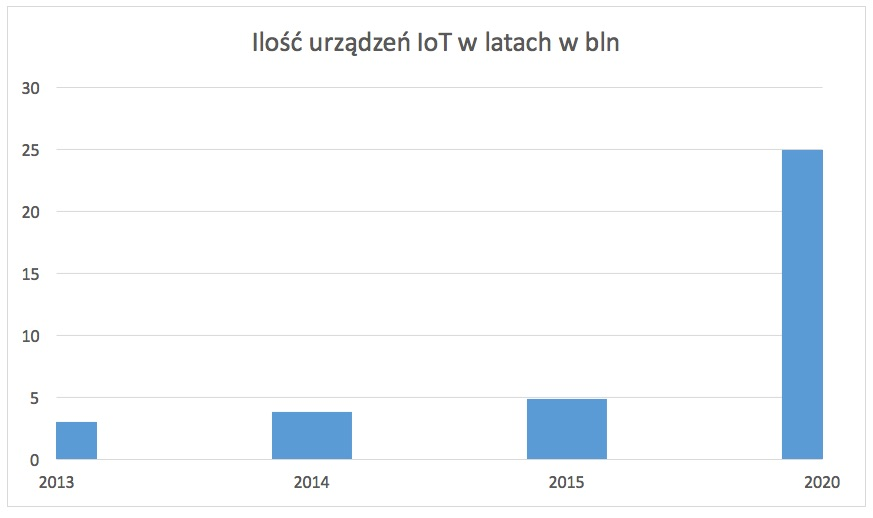
\includegraphics[width=\textwidth]{w}
\caption{Ilość urządzeń IoT, źródło: Gartner, listopad 2014r.}
\label{fig:ilosciot}
\end{figure}
\clearpage
	Pewna część społeczeństwa widzi w~\emph{IoT} szanse, inni boją się, że postępująca cyfryzacja za bardzo rozpowszechnia się w~naszym życiu. Mimo wszystko, liczba urządzeń podłączonych do Internetu wzrasta w~bardzo szybkim tempie i~szacuje się, że do 2020 roku osiągnie ponad 25 mld urządzeń na całym świecie (rys. \ref{fig:ilosciot}).
	Stefan Ferber, na łamach portalu \emph{Harvard Business Review}, twierdzi, że w~2015 roku nie tylko ponad 75\% populacji bedzie korzystać z~Internetu, ale również okolo 6 miliarów urządzeń \cite{harvard}. Możemy do nich zaliczyć smartfony i~laptopy, a~także samochody, fabryki, a~nawet całe miasta \cite{miasta}, gospodarkę wodną czy systemy obronne. IoT wpływa między innymi na projektowanie i~serwis, a~także na zarządzanie zasobami ludzkimi, dzięki czemu stwarza ogromne szanse na „lepsze jutro” w~dziedzinie biznesu. 

\section{Warunki istnienia IoT}
	Jak już wcześniej wspomniano, \emph{IoT} może być rozumiany jako ekosystem, w~którym komunikacja występuje z~udziałem człowieka, lub bez niego. Aby móc wymienić informacje między dwoma przedmiotami, należy spełnić określone warunki.
\begin{figure}[h]
\centering
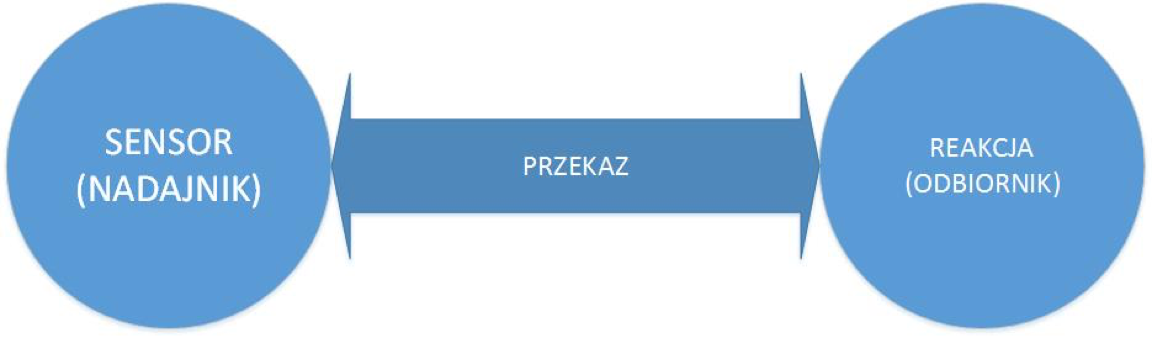
\includegraphics[width=\textwidth]{o}
\caption{Opracowanie własne}
\label{fig:opracowanie}
\end{figure} 
	Pierwszą ważną rzeczą jest fakt, iż przedmiot, który ma wysyłać informacje, musi być wyposażony w~sensor. Dzięki niemu jest w~stanie zebrać potrzebne dane z~otoczenia, aby móc je przekazać odbiorcy (rys \ref{fig:opracowanie}). Jako nadajniki mogą posłużyć smartfony, czujniki wilgotności, temperatury czy ruchu. Różnica między tymi czujnikami a~smartfonami jest taka, iż ze smartfona dane są wysyłane dzięki akcji, którą wyzwala człowiek, a w przypadku czujników dzieje się to automatycznie. Przykładem mogą być modne ostatnimi czasy opaski mierzące tętno, czy liczące ilość wykonanych w ciągu dnia kroków.
	Kolejnym warunkiem, jaki musi być spełniony jest fakt, że przedmiot, który będzie odbierał sygnał przesłany przez nadawcę, musi być w~stanie go odczytać, przetworzyć i~wywołać odpowiednią relację. Przy odbiornikach takich jak komputer czy telefon, przesłana informacja wyświetli się na ekranie. Odbiornikami mogą być również urządzenia, które wykonają określoną czynność, a~nie wyświetlą samej informacji. Przykładem może być układ nawadniania, który automatycznie włączy dopływ wody, bądź kontroler oświetlenia, który o~zmierzchu włączy światło, czy też rolety, które zasłonią się lub odsłonią o~odpowiedniej porze. Bardziej abstrakcyjnymi przykładami mogą być książki, które wyświetlą planowaną datę zwrotu do biblioteki.
	Trzecia rzeczą potrzebną do stworzenia takiej relacji jest sposób komunikacji, czyli to w~jaki sposób dane zostaną przesłane od nadawcy do odbiorcy. Najbardziej popularnymi w~dzisiejszych czasach środkami wymiany danych są WiFi, Bluetooth, oraz mniej znane NFC czy Z-WAVE, które wykorzystywane są w~systemach budynków.  Relację opisanych wyżej trzech rzeczy obrazuje rysunek \ref{fig:opracowanie}.

\section{Korzyści wynikające z~wykorzystania Internetu Rzeczy}
	Tak szybki rozwój technologii i~łączności otwiera drogę na coraz bardziej nowatorskie i~zaawansowane rozwiązania ułatwiające ludziom życie. Największy potencjał w~tej dziedzinie ma inteligentny dom. Dom jest miejscem, w którym czujemy się bezpiecznie i~zawsze możemy do niego wrócić. Nic więc dziwnego, że stale chcemy ułatwiać sobie życie dostosowując otaczającą nas elektronikę do naszych potrzeb.
\begin{figure}[h]
\centering
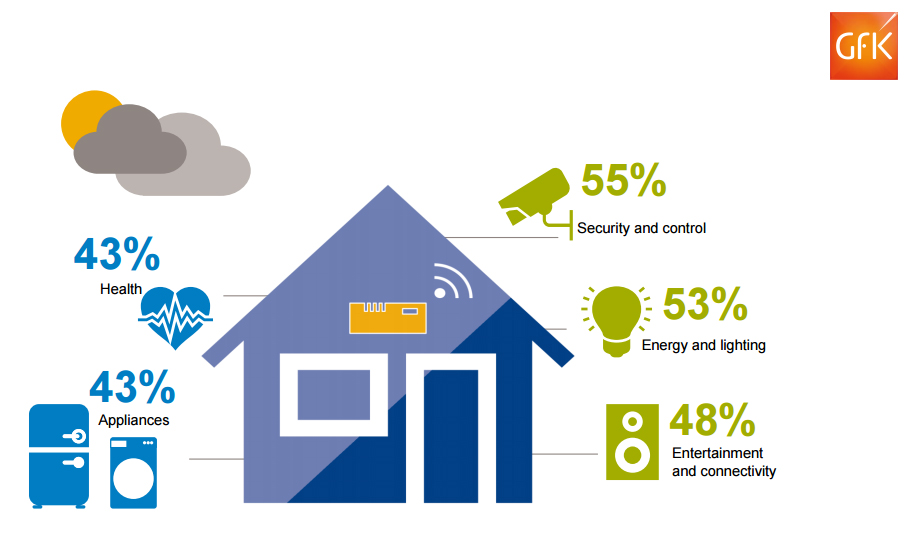
\includegraphics[width=\textwidth]{m_percent}
\label{fig:gfk}
\caption{Raport GfK na temat Internetu Rzeczy}
\end{figure} 
	O ile do niedawna możliwość posiadania inteligentnego domu zarezerwowana była tylko dla osób, które byłyby w~stanie sobie taki dom skonstruować to teraz jest coraz więcej firm które zrobią to za nas. Koncepcja tzw. \emph{smart home} jest najszybciej rozwijającą się ideą w~dziedzinie Internetu Rzeczy. Niemiecki koncern zajmujący się badaniem opinii publicznej GfK przeprowadził w~2015 roku analizę rynku inteligentnych domów. Gwałtowny rowzój technologii, coraz więcej przedsiębiorstw interesujących się tematem oraz prognozy firmy GSMA, która w~2011 roku oszacowała rynek inteligentnych domów na 40 miliardów dolarów~ \cite{Gsma:2011:CMC}, przyczyniły się do powstania raportu GfK. Badaniu poddanych zostało ponad 7.000 respondentów z~7 krajów – USA, Wielkiej Brytanii, Niemiec, Japonii, Chin, Brazylii oraz Korei Południowej. Według przeprowadzonego badania aż 91\% respondentów było świadomych co oznacza idea inteligentnego domu, a~68\% badanych posiadało ogólną wiedzę na ten temat. To bardzo dobry wynik jak na koncepcje, o~której do niedawna w~ogóle się nie mówiło.
	Raport ukazuje również, że 55\% badanych uważa bezpieczeństwo za jeden z~ważniejszych aspektów. Mowa oczywiście o~monitoringu, alarmach i~systemach zapobiegawczych. Jednak rozwiązanie to ma swoje wady, które zostaną dokładnie opisane w~następnym rozdziale.~ \cite{Gfk:2015:CMC}
	Głównym kierunkiem rozwoju jest spotęgowanie relacji pomiędzy człowiekiem, a~przedmiotem, a~to wywołuje potrzebę analizy coraz większej ilości danych. 
	Jest wiele korzyści wynikających z~korzystania z~rozwiązań \emph{IoT}. Zalicza się do nich lepsza kondycja fizyczna oraz zdrowie własne i~bliskich. Ważną rzeczą jest też większe poczucie kontroli nad urządzeniami. Inną korzyścią jest podwyższenie produktywności i~bezpieczeństwa kadry pracowniczej oraz poprawa relacji z~klientem, dzięki zwiększonej komunikacji.
\chapter{Kierunki rozwoju Internetu Rzeczy}

\section{Warunki rozwoju IoT}
	Są trzy poziomy dojrzałości \cite{RP:2015:IOTPL}, dzięki którym możemy zauważyć bezpośrednie korzyści biznesowe. 
\begin{itemize}
\item Pierwszy poziom „Data to Discovery”, mówi o~bazie nowych danych i~ich wykorzystaniu, w~celu  zdobycia informacji o~rzeczach, o~których nie wiedziano dotychczas. Przykładem może być odnalezienie nowych wzorców choroby dzięki informacji z~maszyn medycznych. 
\item Drugim poziomem dojrzałości jest „Data to Decisions”, w~którym mowa o~tym, że na bazie odpowiednich danych można podjąć autonomicznie akcje, na przykład awaryjne wyłączenie urządzenia w~momencie awarii. 
\item Ostatnim poziomem jest „Data To Dollars-Dividents”, gdzie widać korzyść finansową dla firmy bądź szanse jej rozwoju, gdy połączy się dwa wcześniejsze poziomy ze sobą oraz wprowadzi usługi i~produkty innowacyjne.
\end{itemize}
 
	Media społecznościowe wpłynęły znacząco na to jak zaczęto organizować swoje życie, oraz zmieniły one modele biznesowe. Tak samo Internet rzeczy znalazł już swoje miejsce. Można powiedzieć, że jest on etapem rewolucji informacyjnej. Dostarczamy techniki i~narzędzia, dzięki którym możemy budować bazę wiedzy. Na dużych i~szybkich strumieniach danych, nowoczesne urządzenia są w~stanie podejmować odpowiednie decyzje. Sukcesu można się spodziewać, jeżeli wprowadzi się innowacyjne zastosowania w~nowej przestrzeni. 
	Na rozwój IoT miało wpływ wiele rzeczy. Jedną z~nich i~najważniejszą jest miniaturyzacja. Dzięki niej możemy wszędzie umieścić mikroelementy (czujniki, komputery). Ważną rolę odegrała też technologia mobilna, która ciągle się rozwija. Ostatnią znaczącą rolą, bez której IoT by nie istniało jest bezprzewodowa sieć internetowa. 
\section{Idea rozwoju Internetu Rzeczy}
	Niestety istnieje kilka barier rozwojowych dla tematu IoT. Pierwsza to problem zasilania. Każde urządzenie, nawet to, w~którym jest bardzo mocna bateria, wymagać będzie w~końcu podłączenia do prądu. Kolejną barierą jest ilość tylko 4 mld urządzeń, które mogą posiadać adres IPv4 (przy założeniu ze wszystkie będą wykorzystane przez zdresacje IPv4). Aby rozwiązać ten problem należy używać adresacji w~wersji IPv6, który w~obecnej prognostyce rozwoju Internetu powinien być wystarczający. Kolejną przeszkodą, która zostanie przytoczona jest bezpieczeństwo danych i~prywatność. Przekonanie ludzi, że informacje są chronione jest bardzo trudne. Przykładem tego zjawiska są banki. Jeżeli dane między urządzeniami będą tak samo zabezpieczone jak środki na internetowym rachunku bankowym to Internet of Things stanie się bardziej popularny~ \cite{KeyApplications}.
	Dla przeciętnego człowieka internet to połączone w~sieć komputery, które wymieniają się danymi. Internet jest dla niego miejscem czerpania wiedzy, rozrywki, komunikowania się i~wrażania swoich opinii. Jest to dla niego otwarty, częściowo anonimowy wirtualny świat, zupełnie inny od tego w~którym żyje na co dzień. Początki internetu były skromne. Teraz jest to ogromna sieć łącząca ze sobą już nie tylko komputery, telefony czy też urządzenia gospodarstwa domowego. Internet rozrasta się w~tempie wykładniczym – jego rozwój niesie za sobą ogromne korzyści, ale również poważne zagrożenia.
\begin{figure}[h]
\centering
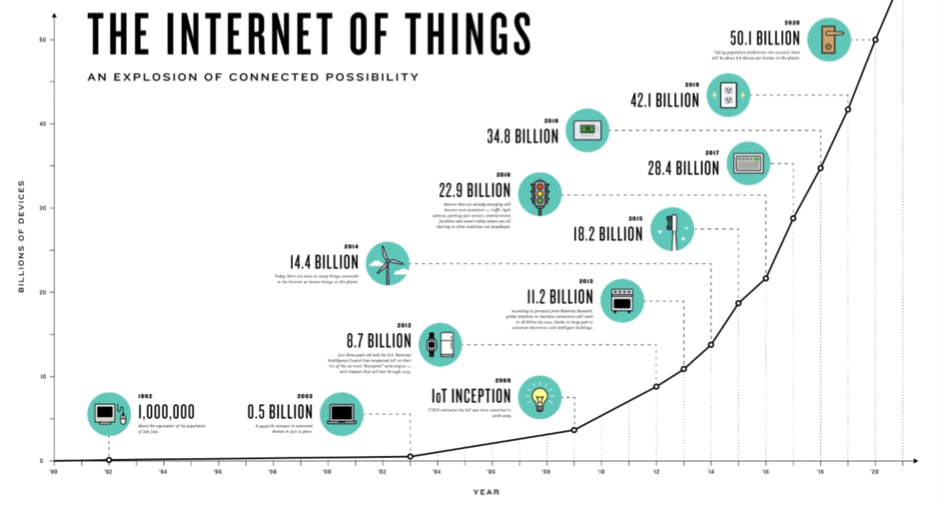
\includegraphics[width=12cm]{m_exp}
\caption{Interet Rzeczy: Rozwój możliwości (IoT: An explosion of connected possibility)~ \cite{Nsr:2015:CMC}}
\label{fig:exp}
\end{figure} 
	Największym motorem napędowym ekspansji Internetu Rzeczy jest chęć ludzi do ułatwiania sobie życia. Najlepszym tego przykładem jest koncepcja tzw. „Inteligentnego Domu”. Już w~tym momencie możemy ustawić pralkę, aby rozpoczęła swoją pracę z~opóźnieniem dzięki czemu możemy wrócić do domu akurat gdy pranie się skończy. Możemy zainstalować przełączniki światła sterowane dźwiękiem, dzięki czemu możemy zgasić lub zapalić światło nie wstając z~łóżka. Mamy czasowe przełączniki, które symulują obecność domowników podczas ich nieobecności, żelazka, które same się wyłączą po pewnym okresie nieaktywności i~tak dalej. Przykładów jest dużo więcej, a~codziennie dochodzą nowe urządzenia, które w~mniejszym lub większym stopniu ułatwiają nam życie w~domu. Jeśli połączymy te wszystkie urządzenia w~jedną sieć zarządzaną centralnie możemy mówić o~inteligentnym domu. Jest on inteligentny na swój sposób – jest zaprogramowany aby zachowywać się w~określony sposób lecz nie jest do końca autonomiczny. Co raz bardziej rozpędzający się postęp technologiczny w~połączeniu z~nieograniczoną ludzką wyobraźnią tworzy mieszankę wybuchową co wcale nie oznacza najgorszego. Wszak dynamit jest teraz kojarzony z~bandytami napadającymi na banki, został wynaleziony w~celu ułatwienia wydobywania naturalnych zasobów Ziemi~ \cite{Rethinking}.
	Internet Rzeczy rozwija się w~wielu kierunkach, nawet w~dziedzinach które w~ogóle nie kojarzą się z~elektroniką. Doskonałym przykładem są tzw.\emph{wearables}, czyli przedmioty osobiste które użytkownik nosi na sobie. Są to na przykład \emph{smart watch'e}, które mają wbudowane moduły łączności bezprzewodowej.  Takie urządzenia mogą mieć dodatkowo wbudowane moduły GPS, co w~teorii może znacząco ułatwić wezwanie pomocy w~odpowiednie miejsce. Jednak taki zegarek może też przysporzyć wielu kłopotów – gdy osoba trzecia uzyska dostęp do danych lokalizacyjnych  może z~łatwością śledzić użytkownika i~wykorzystać tę wiedzę do złych celów. Jeśli włamywacz ma absolutną pewność, że dana osoba znajduje się setki kilometrów od domu to bez większego ryzyka nakrycia może ten dom okraść.
	Na szczęście rynek \emph{wearables} jeszcze raczkuje, a~najwięcej urządzeń mogących tworzyć Internet of Things powstaje w~dziale RTV/AGD. Urządzenia domowe już dawno przyćmiły swoich protoplastów swoją mocą obliczeniową i~możliwościami. Współczesne telewizory nie tylko są w~stanie wyświetlać obraz nadawany z~zewnętrznego urządzenia, ale same potrafią rozkodować sygnał z~anteny. Mają własne systemy operacyjne, które implementują możliwości będące do niedawna ekskluzywną domeną komputerów osobistych. Posiadają przeglądarki internetowe, komunikatory a~nawet gry. Niektóre mają wbudowane kamerki internetowe, a~większość z~nich obsługuje peryferyjne urządzenia rejestrujące. Tutaj znowu pojawia się problem, ponieważ owszem te urządzenia wykorzystywane są do prowadzenia wideo-rozmów ale gdy dostęp do nich uzyska niepowołana osoba stwarza to realne zagrożenie dla domowników, nie mówiąc już o~utracie jakiejkolwiek prywatności.
	Udział sprzętu RTV/AGD w~ekosystemie IoT przekracza 30\%~ \cite{IotWPolsce:2015:CMC}. Nic w~tym dziwnego, skoro cała idea Internetu Rzeczy zrodziła się właśnie w~urządzeniach tego typu. Są to na razie tradycyjne sprzęty użytku domowego, czyli np. skanery, telewizory, urządzenia audio. Nowości na rynku sprzętu elektronicznego, takie jak smart lodówki, stanowią znikomy ułamek całego udziału sprzętu RTV/AGD w~urządzeniach uważanych jako mogące być częścią IoT.

\section{Zagrożenia płynące z~rozwoju IoT}
	Urządzenia, z~których korzystamy na co dzień są co raz bardziej złożone. Ma to na celu oczywiście ułatwienie życia i~umożliwienie dokonywania rzeczy które wcześniej istniały tylko w~sferze fantastyki. 
	Najbardziej niebezpieczne wydają się wspomniane wcześniej \emph{wearables}. z~definicji nosimy je zawsze przy sobie i~to one stanowią największe niebezpieczeństwo dla użytkownika oraz są najbardziej podatne na utratę prywatności. Przykładem nasuwającym się od razu na myśl jest \emph{Google Glass}. Dodatkowo zaciera się granica między rodzajami Rzeczy Internetu – \emph{Google Glass} może być używane do kontrolowania domu, i~osoby trzecie, które uzyskają dostęp do urządzenia, będą w~stanie kontrolować cały dom i~potencjalnie szpiegować domowników.
	To urządzenie może wkrótce zrewolucjonizować rynek urządzeń mobilnych. Jednak niesie to za sobą poważne zagrożenia. \emph{Google Glass} do komunikacji z~siecią może używać albo połączenia \emph{Bluetooth} albo \emph{Wi-Fi}. w~przypadku tego pierwszego potrzebne jest dodatkowe urządzenie służące jako punkt dostępowy dla okularów od internetowego giganta. Druga opcja jest bardziej przystępna, gdyż nie wymaga od użytkownika posiadania przy sobie innego urządzenia mobilnego z~dostępem do sieci. Jednak jak zauważa Roberto Martinez, badacz z~Kaspersky Lab, który przyjrzał się sprawie bezpieczeństwa \emph{Google Glass}, komunikacja \emph{Wi-Fi} naraża urządzenie na ataki hakerów. Martinez i~Juan Andres Guerrero – kolega z~zespołu badawczego – przeprowadzili eksperyment w~monitorowanej sieci. Odkryli, że tylko część danych wymienianych między urządzeniem a~punktem dostępowym była szyfrowana. Badaczom udało się ustalić, że „ofiara” szukała połączeń lotniczych oraz miejscowości turystycznych. Potencjalny haker prawdopodobnie mógłby wyciągnąć jeszcze więcej informacji, gdyby tylko poświęcił na to więcej czasu~ \cite{Abusing}.
	“We admit that it is not a~very damaging vulnerability, but even so, profiling via meta data from Web traffic exchange could become the first step of a~more complex attack against the device’s owner.” - Roberto Martinez
	Kolejnym całkiem nowym na rynku urządzeniem które potencjalnie może przysporzyć właścicielowi kłopotów jest \emph{Galaxy Gear 2} od Samsunga. Jest to tzw. \emph{smartwatch} – zegarek, który potrafi dużo więcej niż tylko wskazać godzinę. Eksperci z~Kaspersky Lab również przyjrzeli się temu akcesorium i~zarówno jak i~w przypadku \emph{Google Glass} jak i~tutaj znaleźli potencjalne zagrożenia dla użytkownika. Pierwszą rzeczą, na jaką zwrócili uwagę badacze był aparat. Samsung dobrze zdawał sobie sprawę, że umieszczanie miniaturowego aparatu w~bardzo małym, niepozornym urządzeniu może narobić komuś szkody. Dlatego zegarek wydaje głośny dźwięk za każdym razem gdy robione jest zdjęcie i~nie umożliwia wyłączenia tej opcji w~żaden sposób. Ma to na celu ostrzeżenie ludzi dookoła, że potencjalnie zostało zrobione im zdjęcie. Jednak pracownicy Kaspersky Lab znaleźli obejście tego zabezpieczenia. Wystarczy tylko uzyskać dostęp administratora (tzw. \emph{root}) co jest trywialnie proste mając fizyczny dostęp do urządzenia i~użyć ogólnodostępnego narządzia \emph{ODIN} od Samsunga. Wyłączając dźwięk migawki nie tylko umożliwiamy właścicielowi zegarka robienie tajnych zdjęć innym osobom, ale też umożliwiamy hakerowi robienie zdjęć właścicielowi, tego co robi i~gdzie jest – bez jego wiedzy.
	Innym problemem \emph{Galaxy Gear 2} jest sposób, w~jaki instalowane są aplikacje. Używane jest do tego oficjalne oprogramowanie od Samsunga – Gear Manager – jednak sposób w~jaki aplikacja wgrywa inne programy do akcesorium pozostawia duży potencjał hakerski. Na zegarku nie wyświetla się żadna informacja o~instalowanym oprogramowaniu, co umożliwia instalowanie złośliwych aplikacji bez wiedzy posiadacza. w~połączeniu z~wiedzą jak ukrywać zainstalowane już aplikacje na systemie Android, na którym \emph{Galaxy Gear} 2 operuje, daje to nieograniczone możliwości dla hakerów.
	Na szczęście są to urządzenia dosyć młode na rynku sprzętu elektronicznego i~zagrożenia związane z~włamywaniem się na nie nie są aż tak powszechne. Jak zaznacza Juan Andres Guerrero na chwilę obecną nie ma żadnych dowodów sugerujących, że wearables są celem hakerów jednak to może się zmienić w~przyszłości, gdy staną się bardziej powszechne.
	“At this time there is no evidence to suggest that wearables are currently being targeted by professional APT actors. However there is a~twofold appeal presented by wearables that make them a~likely future target if they are widely adopted by consumers.  In future the data collected by wearable devices is going to attract new players to the cyber-espionage scene.” -  Juan Andres Guerrero
	Aby „poczuć ducha” inteligentnego domu wcale nie trzeba wydawać dużych pieniędzy – każdy z~minimalną wiedzą informatyczną jest w~stanie samemu stworzyć sobie taki dom, na większą lub mniejszą skalę. Wystarczy komputer i~dobry pomysł, aby przekształcić swoje cztery kąty w~coś wyjątkowego.
	Urządzenia, z~których korzystamy na co dzień są coraz bardziej złożone. Ma to na celu oczywiście ułatwienie życia i~umożliwienie dokonywania rzeczy, które wcześniej istniały tylko w~sferze fantastyki.
	Najbardziej niebezpieczne wydają się wspomniane wcześniej wearables. z~definicji nosimy je zawsze przy sobie i~to one stanowią największe niebezpieczeństwo dla użytkownika oraz stanowią największe zagrożenie utraty prywatności. Przykładem nasuwającym się od razu na myśl jest \emph{Google Glass}. Dodatkowo zaciera się granica między rodzajami Rzeczy Internetu –okulary mogą być używane do kontrolowania domu, i~osoby trzecie, które uzyskają dostęp do urządzenia, będą w~stanie kontrolować cały dom i~potencjalnie  szpiegować domowników.~ \cite{Kaspersky:2014:CMC}
	Niebezpieczeństwa niesione przez IoT można rozpatrywać na dwa sposoby: niebezpieczeństwa związane z~informatyzacją świata konsumenckiego oraz optymalizacją sektora przemysłowego~ \cite{Ks:2014:CMC}. w~czasach rozpędzającego się rozwoju Internetu Rzeczy, ludzie skazani są na informatyzację większości dziedzin życia. Inteligentny sprzęt gospodarstwa domowego, elektroniczne zamki do drzwi lub okien, liczniki energii, itd. Wszystkie te sprzęty niosą za sobą spore niebezpieczeństwo, a~ich przeciętni użytkownicy nie zdają sobie sprawy z~powagi zagrożenia. Bo przecież dlaczego ktoś miałby się bać swojej lodówki? Otóż wszystko wskazuje na to, że niedługo lodówki będą w~stanie gromadzić informacje na temat ich zawartości. Wiedza ta w~niepowołanych rękach może zaszkodzić użytkownikowi. Na pewno nie w~bezpośredni sposób, bo dieta ofiary nie może być wykorzystana np. do kradzieży pieniędzy z~konta bankowego. Umożliwi tzw. profilowanie ofiary. Tak niepozorna wiedza jak to co kto je na śniadanie, w~połączeniu z~innymi, teoretycznie bezpiecznymi informacjami jak np. godzina o~której ofiara rano wstaje (wykradziona ze smartwatch'a) oraz np. ile ciepłej wody zużywa ofiara (wiedza wykradziona z~elektronicznych liczników wody). Tak nagromadzona wiedza, pozornie nieprzydatna z~punktu widzenia hakera, pozwala na dokładną inwigilację ofiary, poznanie jej nawyków oraz sposobu w~jaki żyje stylu życia. Taka wiedza może narobić ofierze wielu problemów gdy znajdzie się w~niepowołanych rękach.

\chapter{Doświadczenia praktyczne}

\section{Wykorzystanie Arduino przy budowaniu własnych projektów}

	Przygodę z~Internetem rzeczy możemy zacząć od kupienia gotowych rozwiązań. Daje nam to możliwość stworzenia inteligentnego domu całkowicie samodzielnie. Zakup przykładowego zestawu inteligentnych żarówek pozwala nam na sterowanie oświetleniem w~całym mieszkaniu za pomocą aplikacji na telefon. Jeżeli zaopatrzymy się w~odpowiedni model żarówki, możemy również zmieniać kolor oświetlenia oraz jego intensywność. 
	Zaopatrywanie się w~gotowe przedmioty ma też swoje wady. Jesteśmy ograniczeni przez producenta funkcjonalnością. Programy obsługujące Inteligentne Rzeczy są pisane pod konkretny ekosystem (Android, iOS, Windows Phone) aplikacja może nie działać na naszym urządzeniu. Narażeni jesteśmy wtedy na dodatkowe koszty - zakup sprzętu, lub konieczność poszukiwania innego, często gorszego rozwiązania. Jako osoba studiująca na kierunku Informatyki postanowiliśmy stworzyć inteligentny przedmiot, który będzie działał tak jak go zaprogramujemy. 
	Na przeciw naszym oczekiwaniom wyszedł Projekt Arduino. Powstał on w~2005 roku we Włoszech. Jest to platforma dla systemów wbudowanych, oparta o~8-bitowe mikrokontrolery Atmel AVR. Płytka posiada ustandaryzowany układ wyjścia-wejścia (ang. input-output circuit, I/O circuit) co umożliwia nam  to korzystanie z~urządzeń zewnętrznych takich jak: czujniki, sterowników, silniki, wyświetlacze itp. Istnieje kilka wersji płytek Arduino, jednak większość z~nich nie wymaga żadnego zewnętrznego programatora. Aby wgrać oprogramowania wystarczy podłączyć mikrokontroler do komputera. Arduino posiada własne darmowe środowisko - Arduino IDE. Ogromną zaletą platformy jest jej popularność. Dzięki niej, w~sieci istnieje duża ilość bibliotek do obsługi różnych urządzeń zewnętrznych. Istnieje także sporo poradników i~przykładów zastosowania mikrokontrolera AVR.
	Jest to idealne środowisko dla programistów, którzy są pasjonatami elektroniki, ale nie lubią konfiguracji programatorów, sprawdzania układów i~instalacji sterowników. Do napisania pierwszego programu i~uruchomieniu go na Arduino wystarczy nam komputer, przewód miniUSB-USB oraz sama płytka. 
	Na początku przygody z~płytką Arduino zazwyczaj nie mamy zbyt wiele sprzętu, który moglibyśmy wykorzystać do stworzenia czegoś użytecznego. Dlatego też pierwszym programem, dzięki któremu zapoznajemy się z~samym językiem programowania oraz samym mikrokontrolerem jest miganie wbudowaną diodą.
	Pierwszym przykładem jest domowa stacja meteorologiczna.
	Jednym z~najprostszych, a~dającym najwięcej satysfakcji projektów jest stacja meteorologiczna, zbudowana przy pomocy Arduino oraz kilku czujników. Poziom zaawansowania układu zależy tutaj od osoby budującej taką stacje. Możemy mierzyć temperaturę oraz wilgotność powietrza za pomocą cyfrowego czujnika DHT11 lub DHT22. Jednak taka prosta stacja to nic innego jak domowy termometr.
	W~inteligentnym domu chodzi o~coś więcej. Wspomniany projekt możemy rozbudować o~kilka dodatkowych sensorów i~stworzyć coś naprawdę fajnego, dorzucając takie funkcjonalności jak: wykrywanie burzy, pomiar ciśnienia, sprawdzanie prędkości oraz kierunku wiatru, jednocześnie wysyłając wszystkie dane do sieci tak, żeby mieć wgląd w~historię pogody. Możemy wykorzystać naszą stację jako centrum informacji dla osób zainteresowanych sportami w~których wiatr odgrywa kluczową rolę np. windsurfing, kitesurfing. 
	Drugim przykładem jest sterowanie oświetleniem.
	Za pomocą Arduino jesteśmy w~stanie sterować oświetleniem w~całym mieszkaniu. Wystarczy, że odpowiednio podłączymy moduły z~przekaźnikiem do sterownika. Możliwości tego rozwiązania są dużo większe niż wspomnianego wcześniej gotowego urządzenia. Tutaj cała konfiguracja i~pole manewru leży w~naszych rękach. Możemy odwzorować sklepową wersję inteligentnej żarówki i~ograniczyć się do centralnego sterowania oświetleniem w~domu z~poziomu aplikacji na komórce lub zaprogramować różne sceny. Jednym kliknięciem możemy ustawić oświetlenie tak by sprzyjało czytaniu książki lub oglądaniu filmów.
	Kolejnym ciekawym rozwiązaniem jest podpięcie całego systemu oświetlenia do sieci i~umożliwienie sterowania przez stronę www. Możemy w~ten sposób na przykład sprawdzić czy napewno zgasiliśmy światło w~domu, będąc akurat w~zupełnie innym miejscu. Oczywiście trzeba uwzględnić zabezpieczenie takiego projektu w taki sposób, żeby osoby niepożądane nie mogły przejąć kontroli nad naszym systemem. Zdalne sterowanie oświetleniem daje nam możliwość symulowania obecności w~domu gdy jesteśmy np. na wczasach. Możemy zdalnie włączać i~wyłączać światło, innym sposobem jest automatyzacja i możliwość~ustawienia godziny w~których nasz dom będzie zapalał i~gasił oświetlenie.
	W 2014 roku powstała strona na której można było sterować oświetleniem świątecznym rozwieszonym na domu, jednocześnie mieliśmy podgląd online dzięki któremu na żywo obserwowaliśmy efekty. 

\section{Projekt inteligentnego nawadniania roślin}
	Pamięć o~podlewaniu kwiatów domowych nigdy nie była naszą mocną stroną. Postanowiliśmy więc stworzyć system, który będzie nas informował drogą mailową o~potrzebie nawodnieniu rośliny. Chcieliśmy również zbierać informacje o~temperaturze, wilgotności powietrza i~poziomie wilgotności gleby. Wszystkie dane wysyłaliśmy na serwer i~dzięki stronie internetowej mogliśmy analizować wyniki które ułatwiły nam wyciągnięcie wniosków. 
	Pierwszym krokiem jaki wykonaliśmy to skompletowanie listy rzeczy które były niezbędne do wykonania tego systemu. Należą do nich: 
\begin{itemize}
\item Płytka Arduino UNO: 2,7\$
\item Sensor wilgotności gleby: 0,86\$
\item Sensor temperatury i~wilgotności powietrza: 3,01\$
\item Moduł Wifi: 2,70\$
\item Zestaw kabli i~rezystorów: 2,00\$
\item Płytka stykowa dedykowana do Arduino: 1,31\$
\end{itemize}
	Wartość takiego zestawu na polskim rynku wynosiłaby około 130 PLN. Jednak w~celu zminimalizowania kosztów, zakupu dokonaliśmy w~serwisie AliExpress. Dzięki temu wydaliśmy około 54 PLN (14\$ przy kursie dolara wynoszącym 3,84 PLN).
	Przed przystąpieniem do składania projektu musieliśmy zainstalować IDE (ang. Integrated Development Environment) czyli zintegrowane środowisko do pisania programów, dzięki któremu będziemy mogli wgrywać programy na naszą płytkę. Następnie sprawdziliśmy czy wszystkie sensory działają poprawnie. Zaczęliśmy od podstawowego czujnika DHT11. Jest to układ odpowiadający za pomiar temperatury i~wilgotności powietrza. w~celu sprawdzenia napisaliśmy prosty program wykorzystujący bibliotekę ‘’DHT.h’’. Po podłączeniu zgodnie z~opisem sensora nie byliśmy w~stanie odczytać poprawnych wartości. Po głębszej analizie okazało się, że czujnik który dostaliśmy ma inaczej poprowadzone PINy (info). Kolejną rzeczą która musieliśmy sprawdzić to podłączenie sensora wilgotności gleby do naszej płytki. Po wstępnej analizie danych z~czujnika, porównując wyniki z~innymi użytkownikami tego samego czujnika uznaliśmy, że zachowuje się on prawidłowo. Ostatnim krokiem przygotowawczym było sprawdzenie modułu WiFi. Pozornie najtrudniejszy moduł nie sprawił nam najmniejszych problemów. Wszystko działało poprawnie i~mogliśmy zabrać się za tworzenie inteligentnego systemu nawadniania roślin.
	Po sprawdzeniu każdego czujnika z~osobna mogliśmy przystąpić do pracy. Musieliśmy tylko napisać program który będzie obsługiwał wszystkie moduły naraz. W~pierwszej kolejności podłączyliśmy czujniki odpowiadające za pomiar temperatury, wilgotności gleby i~powietrza. Następnie zajęliśmy się konfigurowaniem połączenia sieciowego. Nasz program sprawdzał wszystkie pomiary trzy razy w~trakcie doby – w~nocy o~godzinie 00:00, o~ 8:00 nad ranem oraz popołudniu o~godzinie 16:00. Dane za każdym razem wysyłane były na serwer. Na rysunku [x] przedstawiony został wykres przedstawiający dane z~trzech dni.

\begin{figure}[h]
\centering
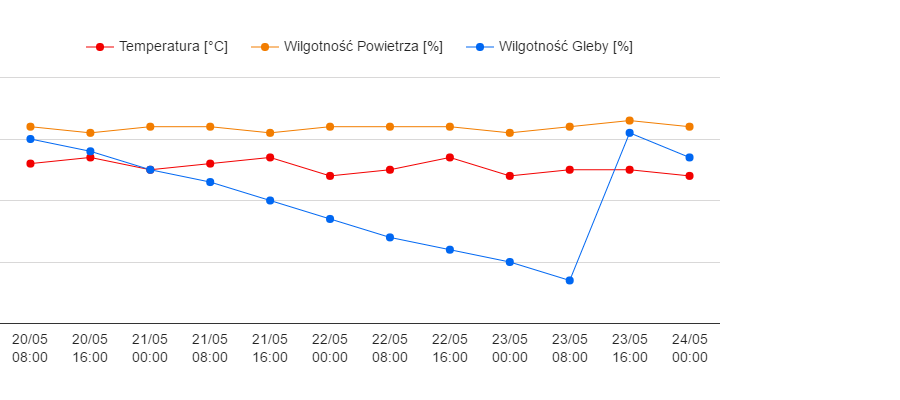
\includegraphics[width=\textwidth]{pawel_wykres}
\caption{Dane z~czujników przedstawione na wykresie, źródło: Opracowanie własne}
\label{fig:iot}
\end{figure}

	Ostatnim krokiem było dodanie powiadomień na maila. Skorzystaliśmy z~gotowego rozwiązania PushingBox (źródło). Jest to dedykowane rozwiązanie dla urządzeń z~dziedziny Internet of Things. Posiada zaimplementowane już rozwiązania między innymi na Arduino.   Wystarczy wykorzystać kod udostępniony przez twórców na stronie i~wdrożyć go w~swoim rozwiązaniu. System informował nas drogą mailową gdy wilgotność gleby spadała poniżej 10%. Na załączonym wykresie [x] można zaobserwować tę zależność. 
\section{Budowa własnego systemu monitoringu}

	Wygodny nadzór nad domem podczas nieobecności do niedawna kojarzył się z~czymś ekskluzywnym. Powszechnie monitoring znajdował się jedynie w~bogatych domach. Jednak z~tak szybkim postępem technologicznym na tego typu luksusy może pozwolić sobie niemalże każdy, praktycznie zerowym kosztem. Większość ludzi posiada jakiś stary, nieużywany telefon komórkowy z~aparatem. Można go wykorzystać jako kamerę IP, dostępną w~sieci lokalnej domu. Specjalne oprogramowanie będzie przesyłać obraz z~dobrze umiejscowionego telefonu do serwera. To może być dowolne urządzenie, jednak na potrzeby naszego eksperymentu będzie nazywany serwerem. W~naszym przypadku użyliśmy 2 aparatów i~laptopa~ \cite{Learning}.
	Za strumieniowanie wideo z~kamery odpowiedzialny jest program IP Webcam1. Aplikacja jest dostępna za darmo, z~możliwością wykupienia wersji pro. w~cenie ok. 12 zł znajdują się dodatkowe funkcje:
\begin{itemize}
\item Integracja z~Taskerem,
\item Konfigurowalny UI,
\item Bezpośredni skrót na ekranie głównym do uruchomienia aplikacji,
\item Brak znaku wodnego,
\item Brak reklam,
\end{itemize}
	To niewielki koszt w~porównaniu z~tym, co aplikacja ma do zaoferowania. Autor programu, Pavel Khlebovich, do wersji pro  podchodzi bardziej jak do dobrowolnej dotacji.
	IP Webcam posiada ogrom funkcji. Oprócz najważniejszej, czyli wystawiania zwykłego interfejsu kamery IP, sama w~sobie posiada funkcję serwera, i~to bardzo przemyślanego. Na wstępie zaskakuje ilość sposobów w~jaki można odbierać obraz i/lub dźwięk z~urządzenia. Można też zapisywać pliki w~archiwum, albo skonfigurować Taskera. Wszystko jest zrobione w~Bootstrap'ie i~działa bardzo dobrze na prawie każdym urządzeniu, dzięki możliwości wyboru sposobu transmisji.
	Ma to niestety podstawowy problem. Ciężko mówić o~monitoringu, mając obraz z~jednej kamery. Wiele kamer oznacza wiele serwerów, każdy nadający obraz tylko ze swojego aparatu. Aby będąc na urlopie podejrzeć obraz z~domu, należałoby zalogować się na każdą kamerę z~osobna, co w~przypadku większej ilości kamer byłoby zupełnie niepraktyczne. Zaprogramowaliśmy serwer w~technologii Meteor, który odbiera sygnał z~wielu kamer, inaczej, zapisuje migawki do pliku i~serwuje je klientowi~ \cite{Started}.
	Aby to wszystko było możliwe najpierw zainstalowano \emph{Meteora}. Po początkowych nieudanych próbach uruchomienia frameworka na wirtualnej maszynie VirtualBox + Vagrant spowodowanych brakiem sympatii sterownika MongoDB do montowanych folderów, postawiliśmy serwer na Windowsie 8.1. Główną wadą tego rozwiązania był brak programu npm, co stanowiło spory problem, gdyż najlepszy naszym zdaniem sterownik do kamer IP jest modułem Node.js. Jednak wszystko jest możliwe z~odrobiną hacks'ów. z~pomocą przyszedł moduł meteorhacks/npm, który wbrew nazwie w~odpowiedni sposób dodaje obsługę npm do Meteora, co zresztą potwierdzają doświadczeni programiści~ \cite{Npm:2014:CMC}.
\begin{figure}[h]
\centering
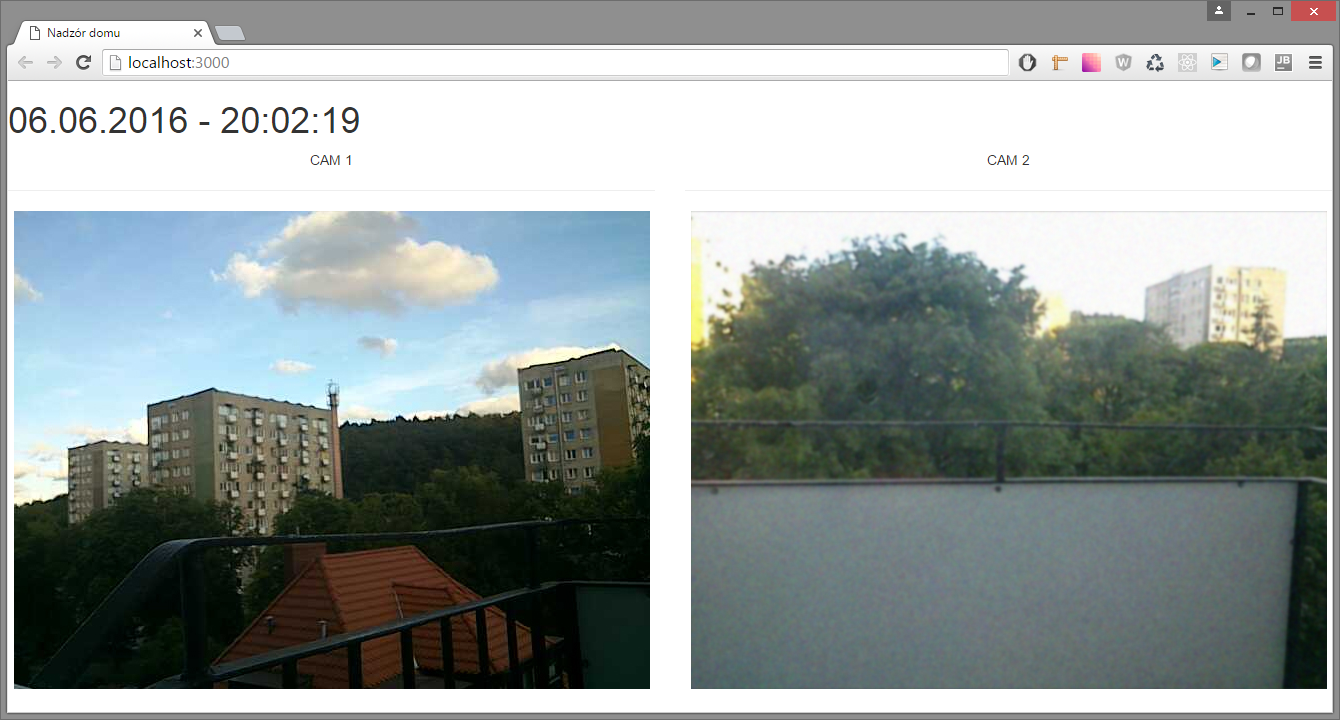
\includegraphics[width=12cm]{m_cam}
\caption{Działający system monitoringu.}
\label{fig:cam}
\end{figure} 
	Potrzebna była jeszcze tylko aplikacja do obsługi naszego ustawienia. z~założenia aplikacja miała obsługiwać wiele kamer, i~to w~dodatku wyświetlać obraz na dowolnym urządzeniu w~dowolnym miejscu. Zatem nie było mowy o~strumieniu na żywo, gdyż rozmiar przesyłanych danych byłby zbyt wielki. Postawiliśmy na prostotę: serwer co sekundę odpytuje wszystkie kamery o~zrzut ekranu. Zapisuje je potem do odpowiednich plików i~wysyła je do klienta, gdzie stanowią one zwykłe obrazki okraszone Bootstrapem dla obsługi urządzeń mobilnych. Obrazki zmieniające się co sekundę dają wrażenie oglądania nagrania na żywo, co technicznie jest prawdą.
	Wiele problemów sprawił też sam node-cam, który jest w~wersji 0.0.1 i~sam autor przestrzega przed tym, że projekt nie jest ukończony. Jednak spodobało nam się proste API i~dzięki wspólnemu wysiłkowi udało nam się skonfigurować ten moduł rys \ref{fig:cam} . 

	Niskie tempo odświeżania rekompensuje fakt, iż możemy podłączyć wiele kamer i~mieć odczyt na żywo z~każdej z~nich. w~naszym przypadku całkowicie zerowym kosztem stworzyliśmy system nadzoru domu, do którego można się zalogować. Do zabezpieczenia aplikacji użyliśmy standardowej autoryzacji poprzez HTTP, której obsługę do Meteora dodaliśmy przy pomocy modułu Jabbslad/basic-auth.

\section{Budowa inteligetnego oświetlenia}

	Budowa systemu oświetlenia, miała na celu znaczące obniżenie kosztów energii elektrycznej oraz prostotę i~użyteczność które to wspierałyby nasze \emph{wrodzone lenistwo}. We wszystkich pokojach w~całym mieszkaniu wliczając łazienkę i~korytarz. Jak mawiał klasyk, \emph{"Do zrobienia rzeczy trudnej wybrałbym osobę leniwą, gdyż taka to właśnie osoba znajdzie najprostszy sposób aby to wykonać} \cite{gates}. w~myśl owej zasady, postanowiliśmy kontrolować oświetleniem za pomocą specjalnych sterowników WiFi sprzęgniętych z~aplikacją na smartfony/tablety oraz zdalnego kontrolera RGB, aby móc kontrolować oświetleniem w~całym domu za naciśnięciem jednego \emph{kciuka}. 
	Źródłem światła w~tym przypadku postanowiliśmy użyć wydajnych i~energooszczędnych taśm LED'owych opartych o~najnowsze diody 5760 oraz w~przypadku pokoju dla młodzieży taśm z~diodami 5050 RGB. w~połączeniu z~wyżej wymienionymi sterownikami WiFi będą duszą naszego projektu. Całość będzie sterowana zdalnie z~dwu źródeł, sensorycznego kontrolera zdalnego rys \ref{fig:led1}, \ref{fig:led2}, \ref{fig:led3} oraz/i aplikacji zainstalowanej na smartfonie rys . 
\begin{figure}[h]
\centering
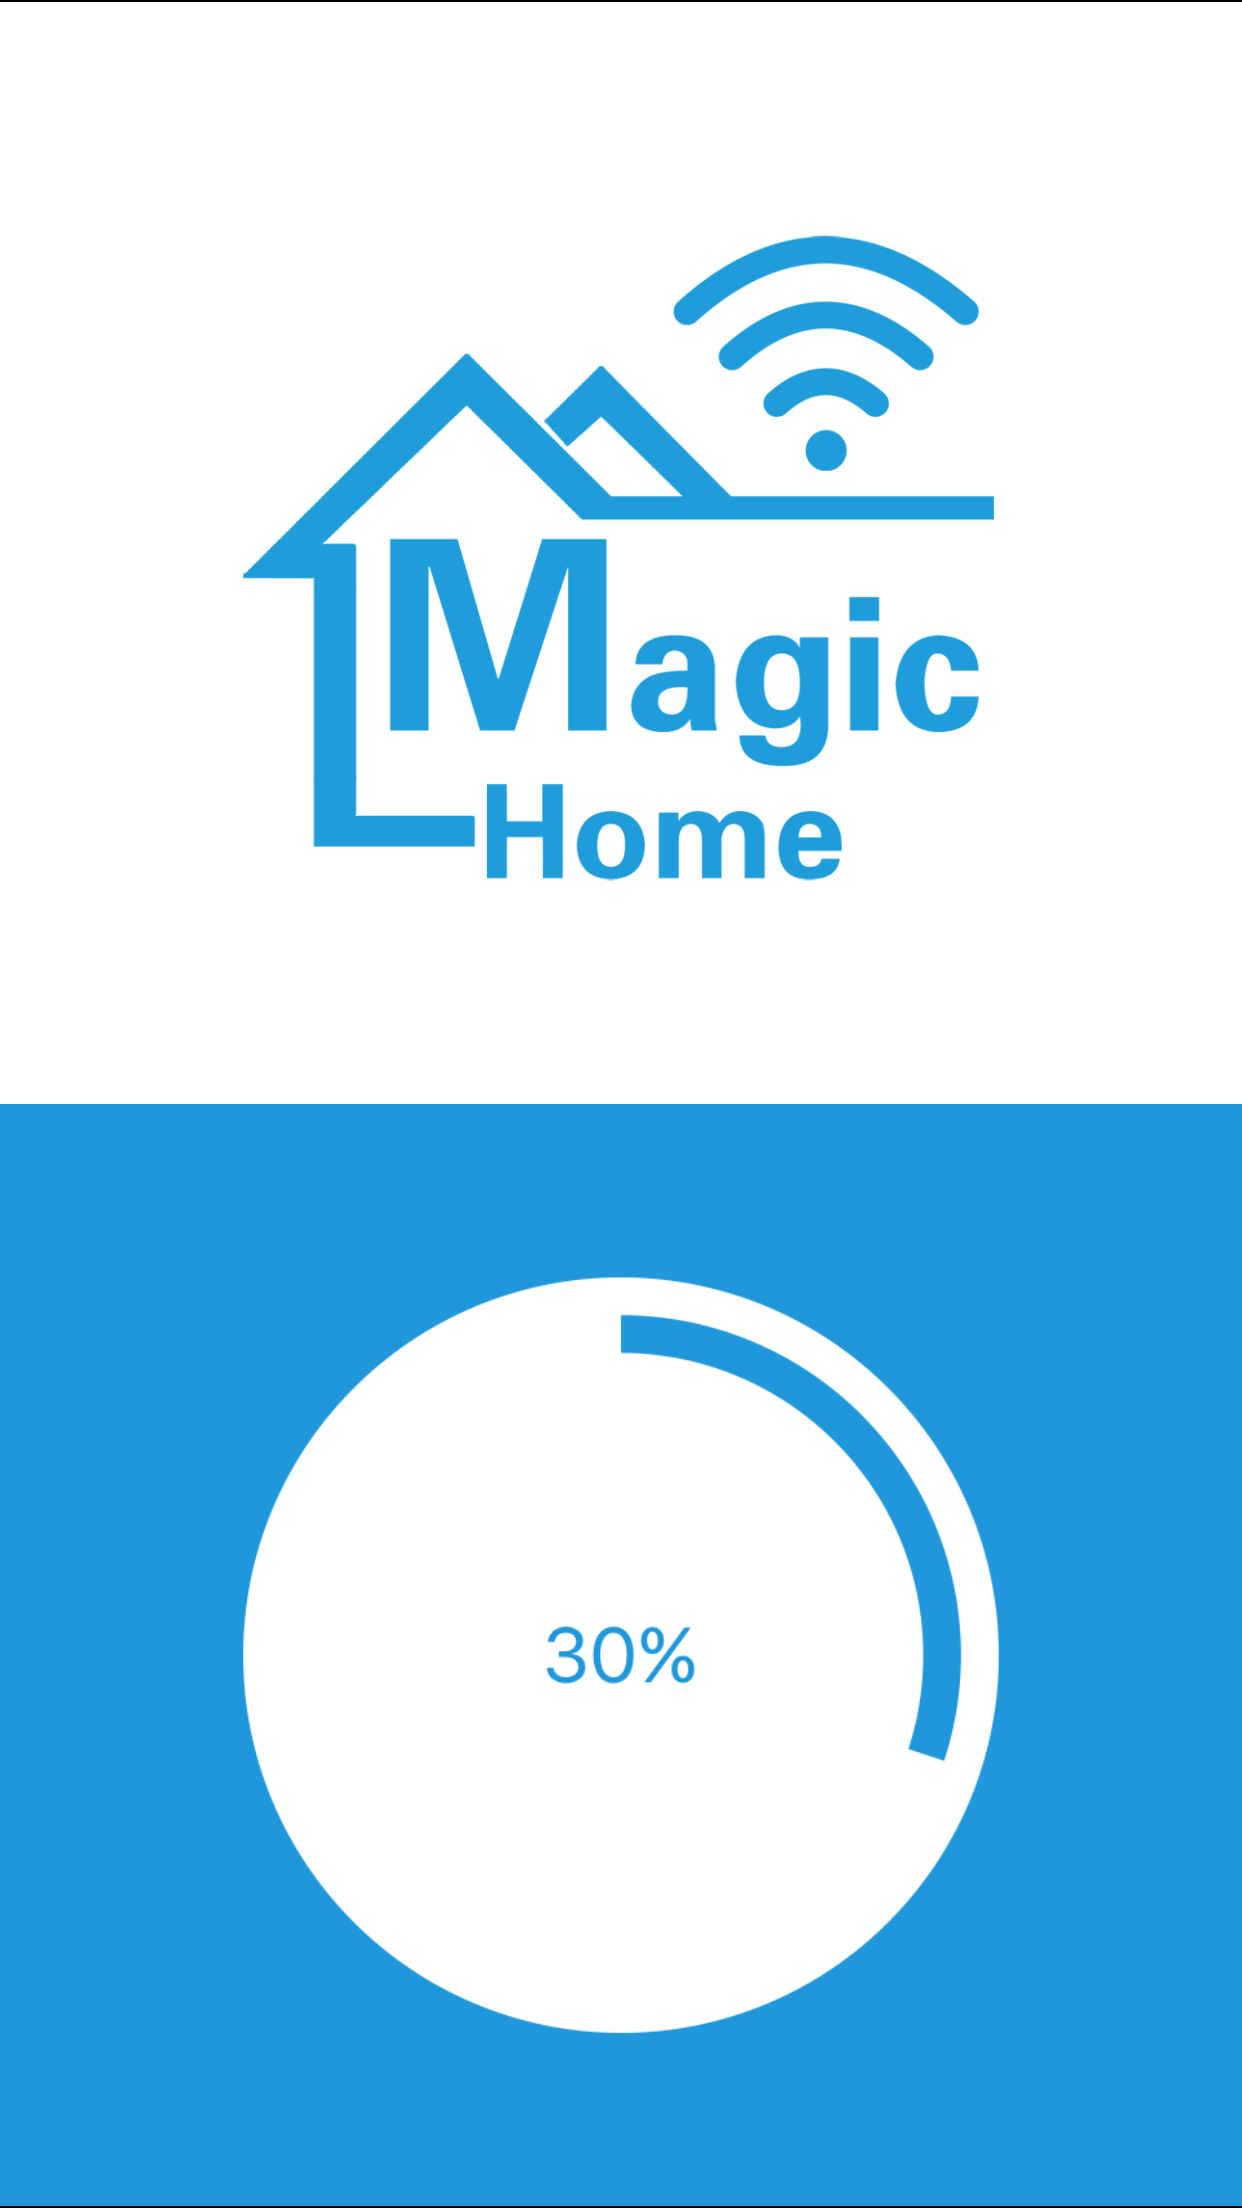
\includegraphics[width=4cm]{magic}
\caption{Aplikacja MagicHome . Opracowanie własne.}
\label{fig:magic}
\end{figure}
	Niestety nie obyło się bez problemów \emph{"wieku niemowlęcego"} projektu, gdyż inicjalnie mieliśmy bazować na sterownikach firmy \emph{"Milight} które niestety nie sa pozbawione wad... Jednakże po dłuższych poszukiwaniach dobraliśmy sterowniki firmy \emph{"Fancy Lighting"}, które to spełniały założenia projektowe naszego rozwiązania. Tradycyjnie w~celu obniżenia kosztów przedsięwzięcia wszystkie komponenty zostały zakupione u~źródła najtańszej produkcji światowej czyli w~Chinach na portalu \emph{Aliexpress.com}.
	W skład wszyskich potrzebnych do budowy zdalnego sterowania oświetleniem komponentów wchodzą:
\begin{itemize}
	\item Taśmy LED'owe \emph{Warm yellow light} oraz \emph{RGB} 8 taśm po 5m każda -> 30\$
	\item sterowniki WiFi szt. 5 -> 50\$
	\item zasilacze 220V->12V -> 20\$ 
	\item kontroler (pilot) oświetlenia RGB -> 8\$
	\item aplikacja \emph{MagicHome} rys \ref{fig:magic} -> 0\$ aplikacja jest darmowa!
\end{itemize}

	Największymi możliwościami jednak dysponuje sterownik WiFi \emph{"Fancy Lighting"} gdyż pozwala nam na kompletne sterowanie z~aplikacji \emph{MagicHome}, którą to mamy dostępną pod większość systemów mobilnych (\emph{IOS, Android, etc}). Jest to najbardziej wygodna funkcjonalność z~jaką do tej pory sie spotkaliśmy. Pozwala na pełną kontrolę oświetlenia w~całym domu jak i~grupowania sterowników w~obrębie jednego pomieszczenia (\emph{np mozemy oddzielnie zapalić oświetlenie aneksu kuchennego oraz połączonego zeń pokoju}). Sam sterownik posiada również pare innych ciekawych funkcji zaimplementowanych inicjalnie (\emph{out of the box}), pierwszą jest możliwość uruchomienia zaprogramowanej przez nas symulacji "pobytu" podczas naszej nieobecności. Jest to skrypt który możemy uruchomić podczas naszego wyjazdu i~każdego wieczoru będzie o~zmierzchu zapalał i~gasił światła w~zdefiniowanych wcześniej grupach \emph{"duzy pokój", "mały pokój", "kuchnia", etc.} co pozwoli na zmylenie potencjalnych włamywaczy obserwujących nasze mieszkanie.

	System posiada również tzw. \emph{party mode} czyli wbudowany system mikrofonów i~podczas puszczania muzyki możemy dla przykładu zamienić duży pokój w~salę taneczną z~piękną iluminacją świetlną która reaguje na puszczane dźwięki.

	Jak widać na przedstawionym zestawieniu powyżej, zestaw nie jest rażąco drogi oraz w~wersji podstawowej funkcjonalności jakoś mocno skomplikowany do wdrożenia, jeśli natomiast będziemy chcieli zaimplementować więcej funkcjonalności to w~tym momencie ogranicza nas tylko nasza wyobraźnia.

\begin{figure}[h]
\centering
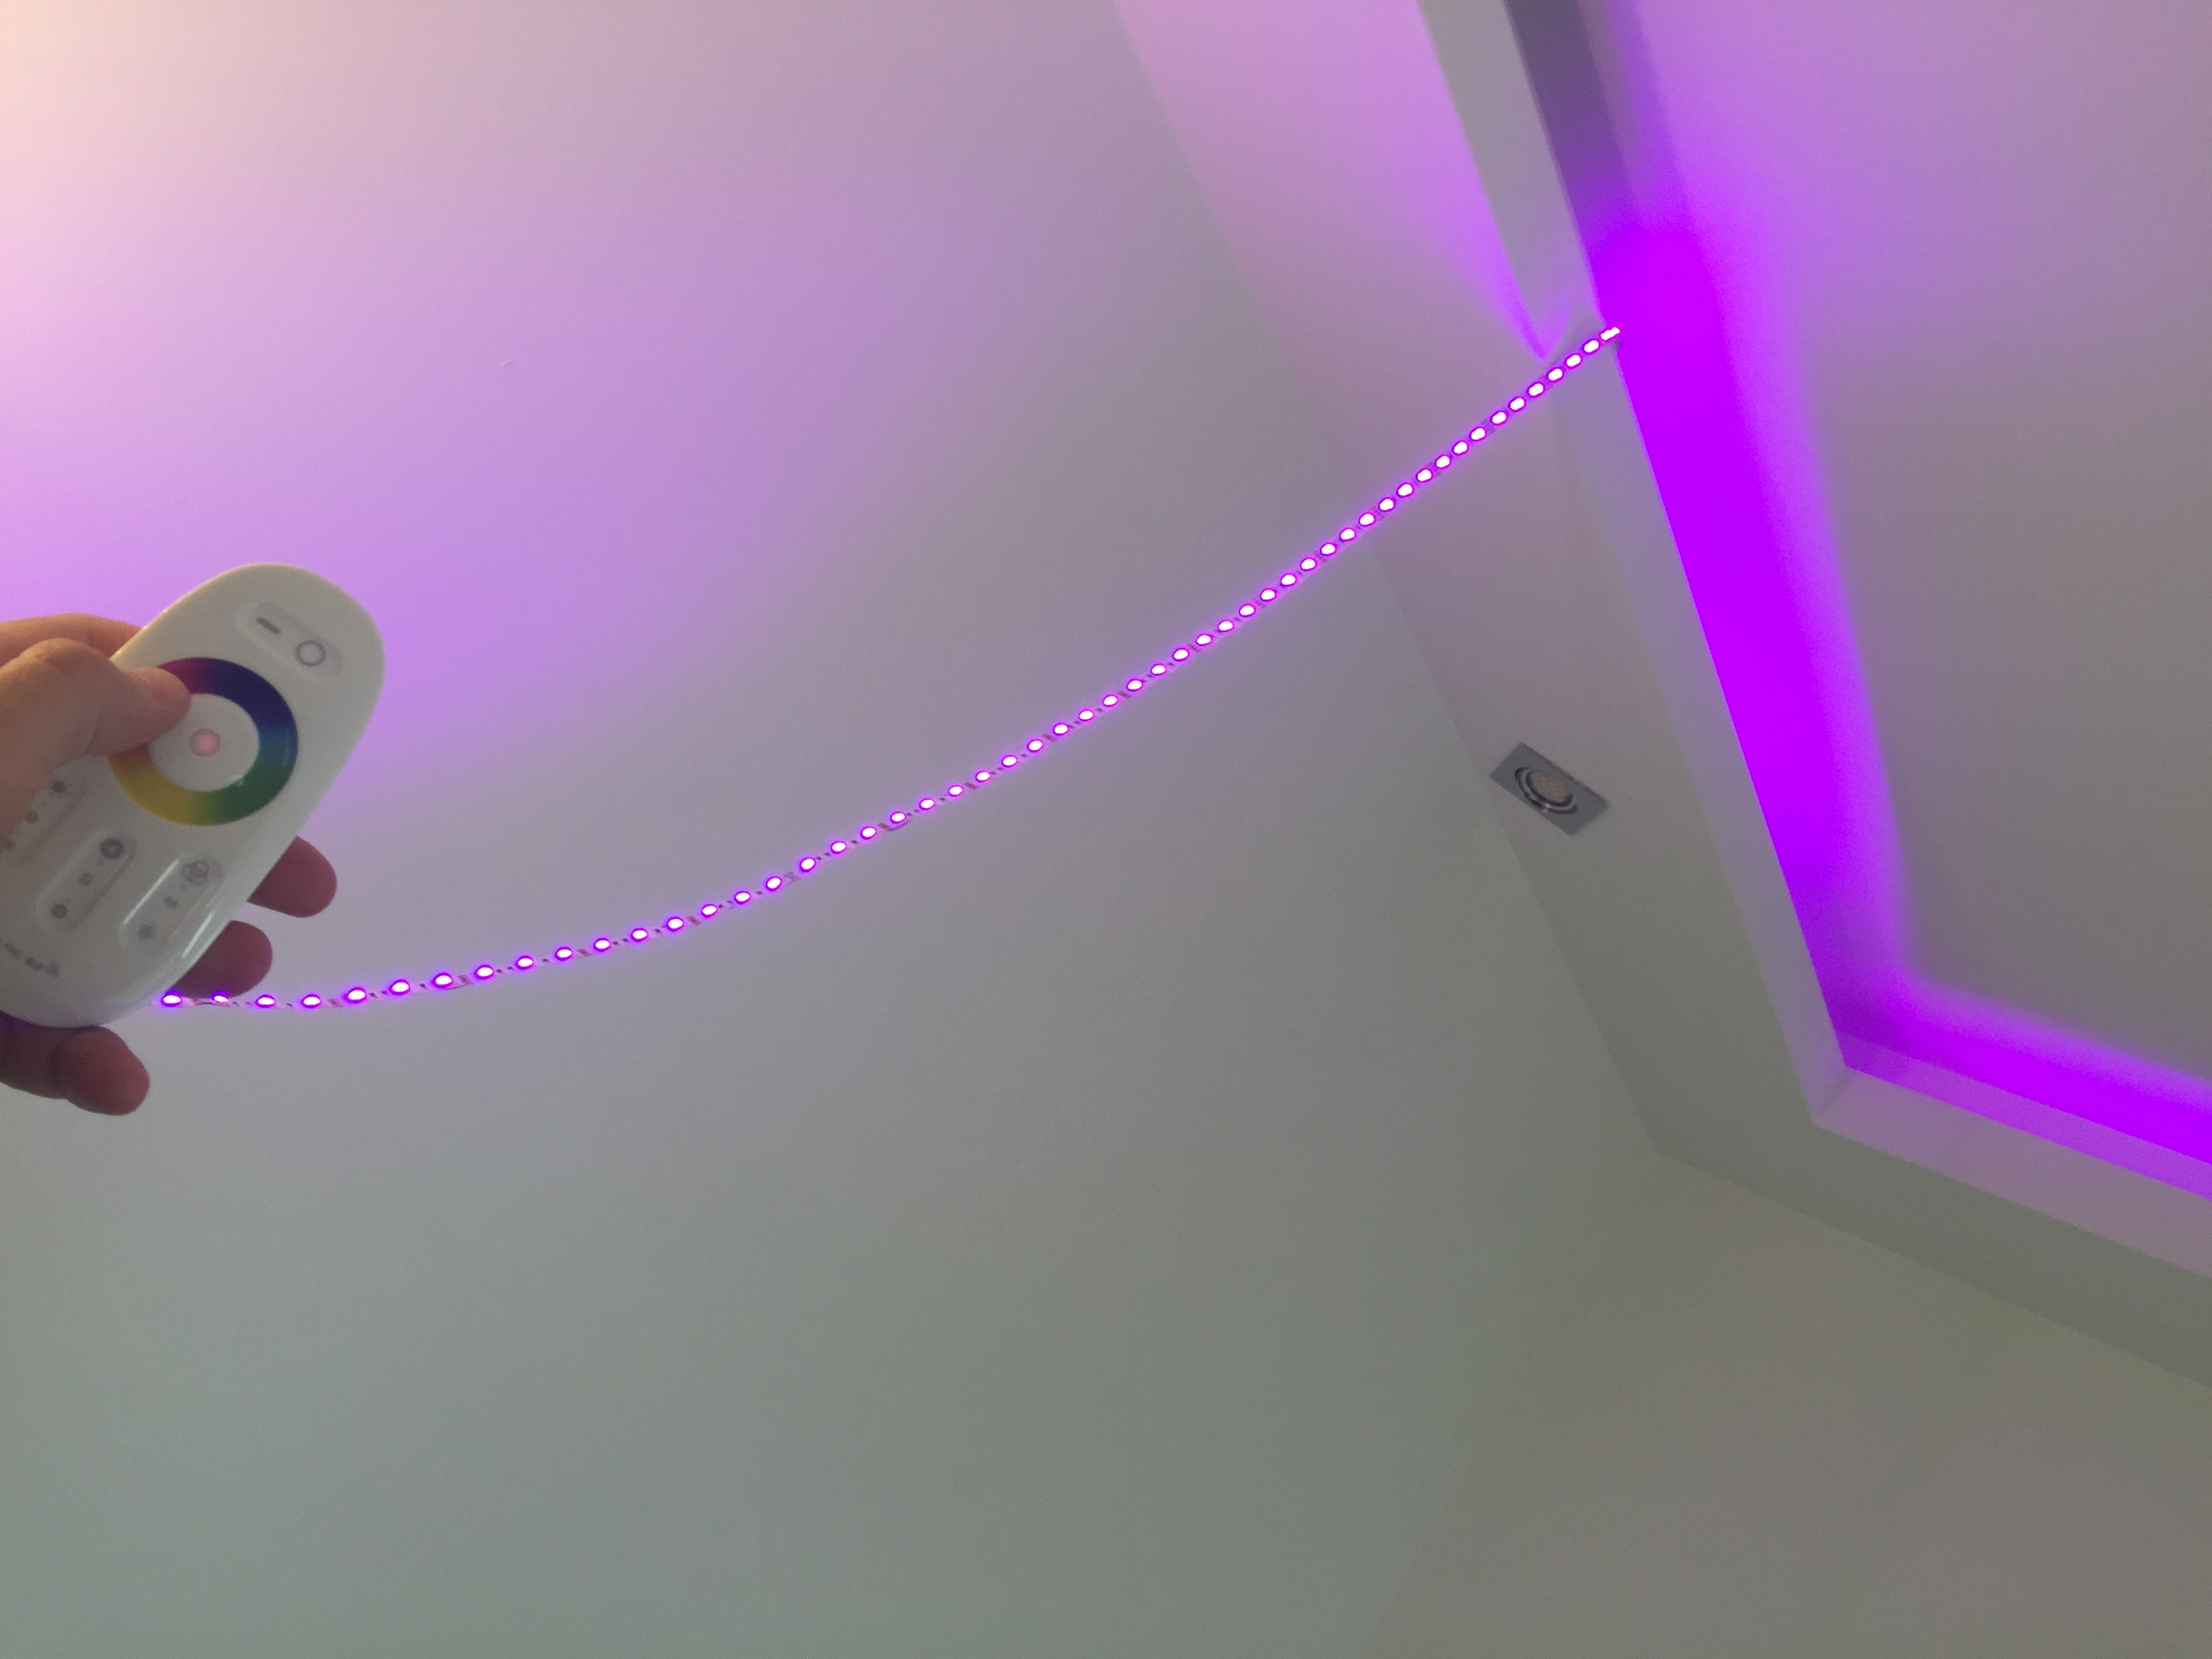
\includegraphics[width=6cm]{led1}
\caption{Oświetlenie RGB oparte o~kontroler. Przykladowy kolor 1. Opracowanie własne.}
\label{fig:led1}
\end{figure} 
\begin{figure}[h]
\centering
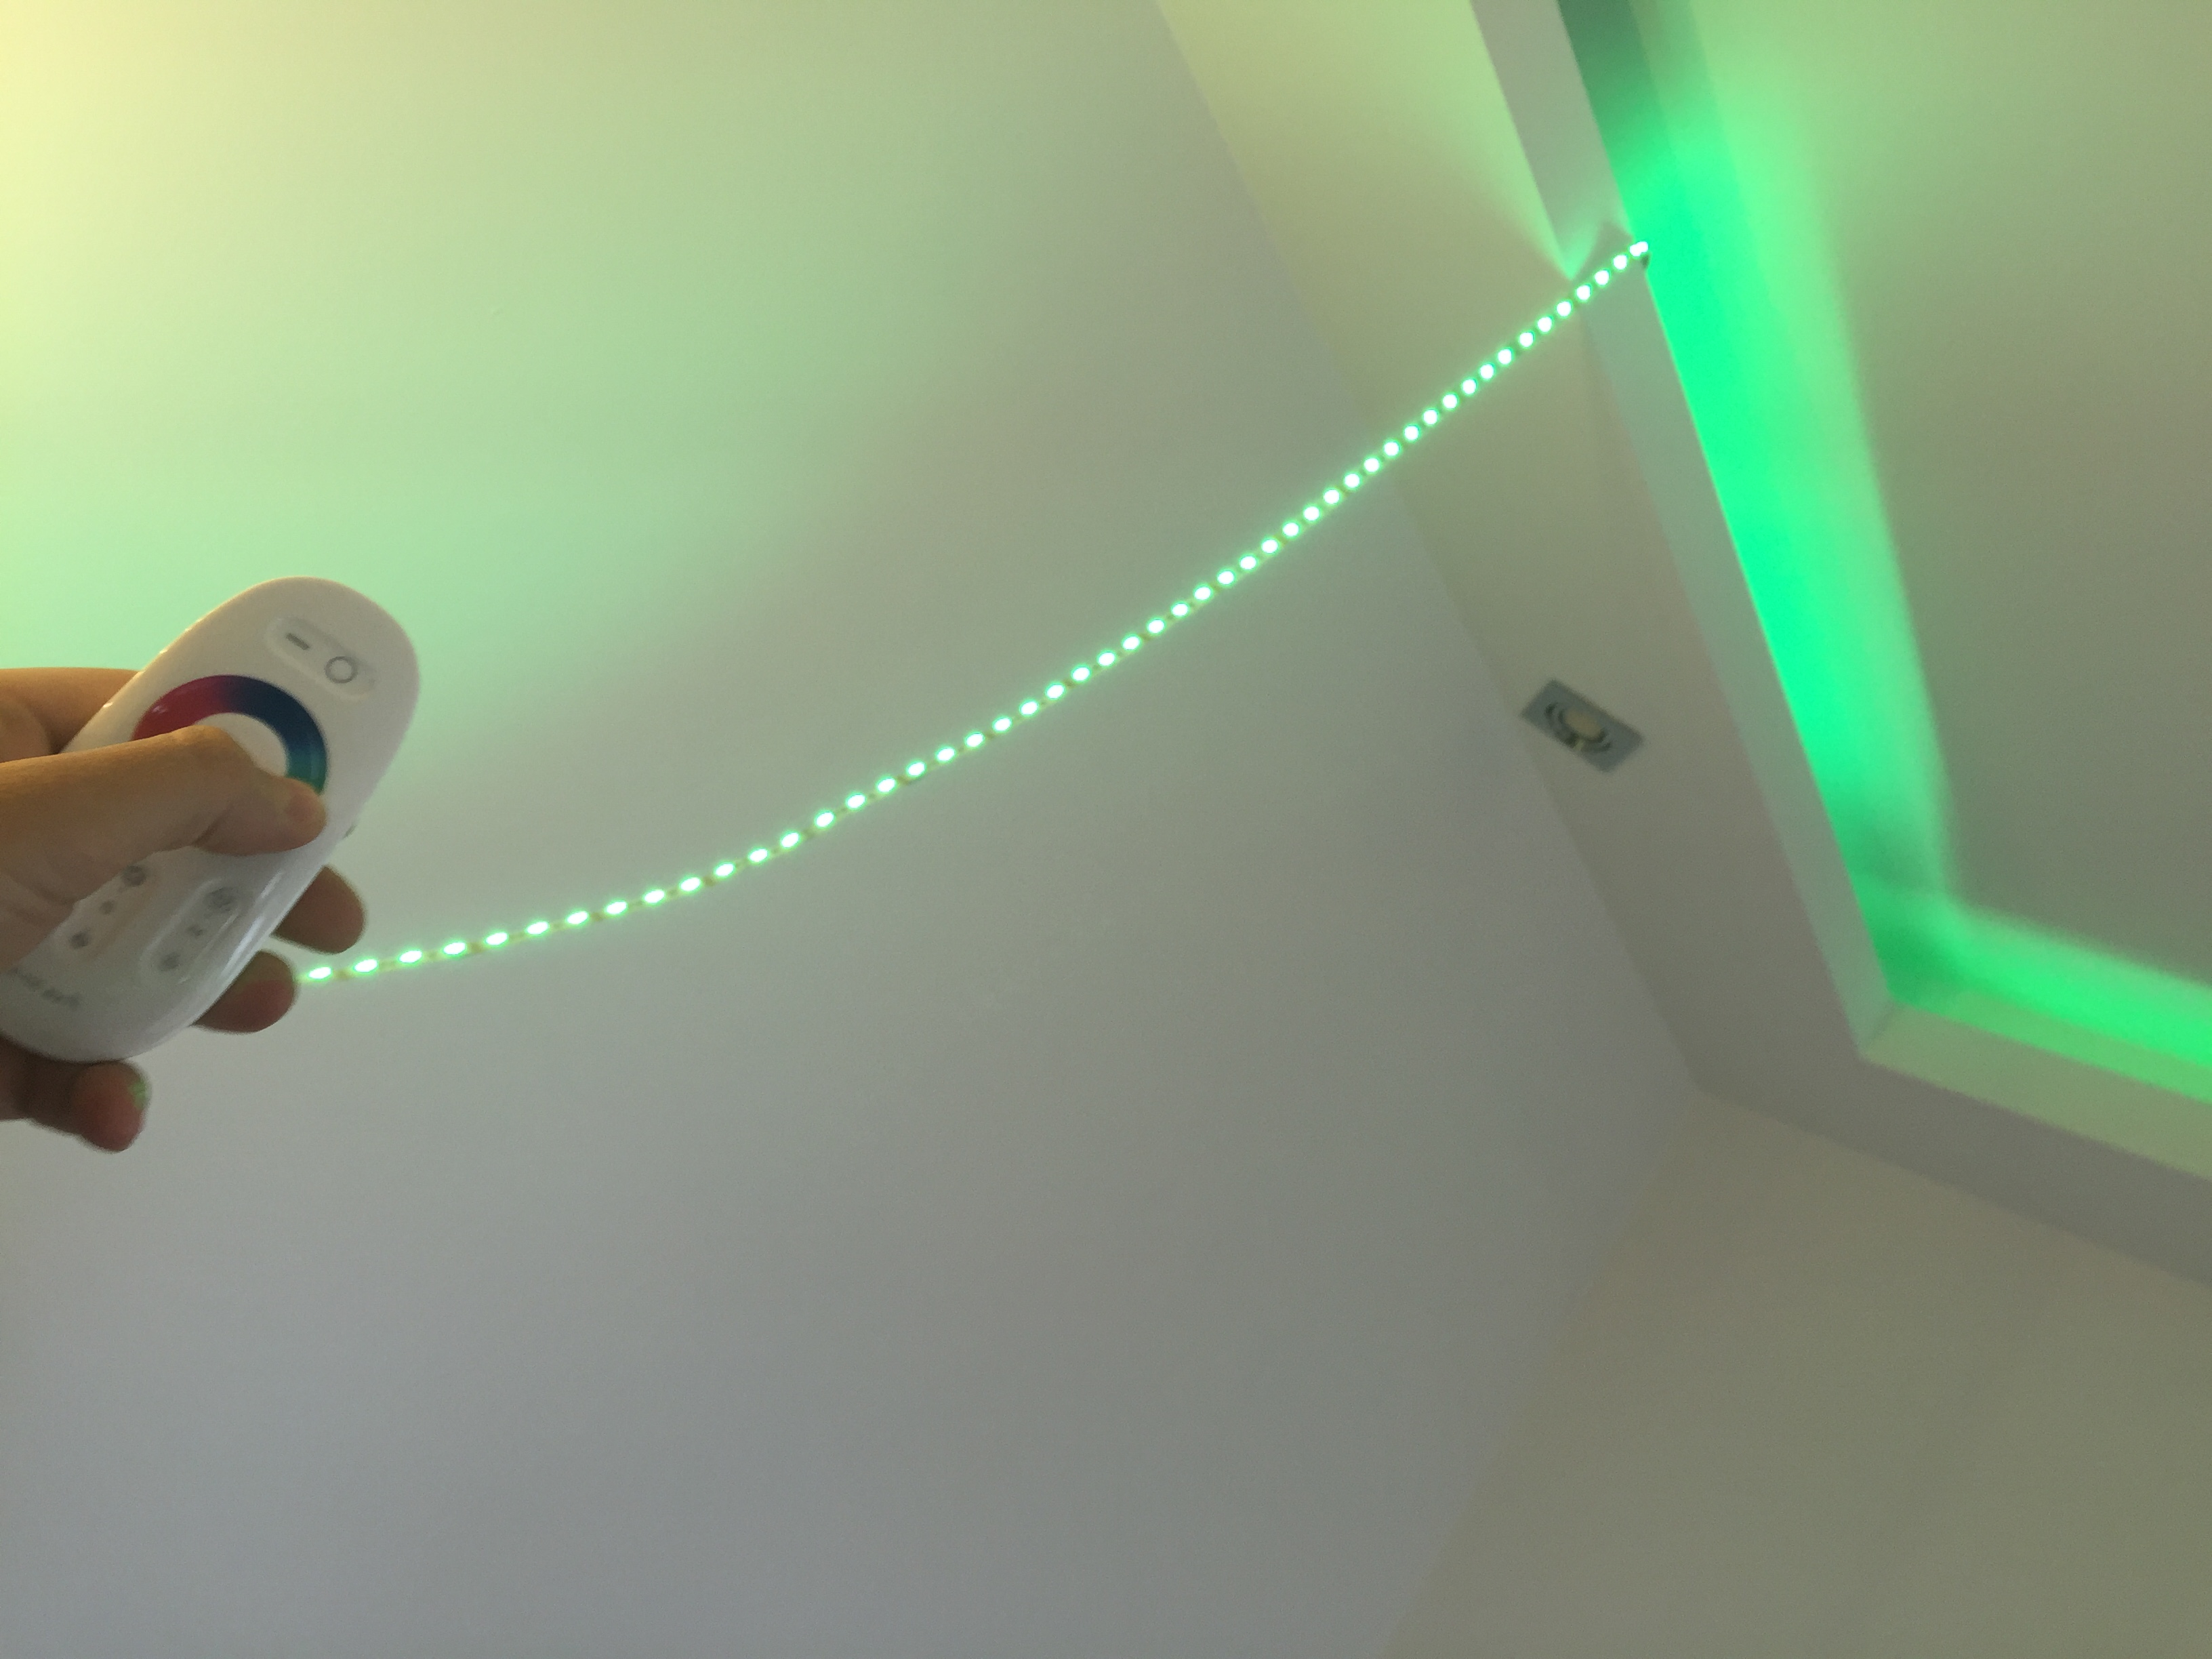
\includegraphics[width=6cm]{led2}
\caption{Oświetlenie RGB oparte o~kontroler. Przykladowy kolor 2. Opracowanie własne.}
\label{fig:led2}
\end{figure} 
\begin{figure}[h]
\centering
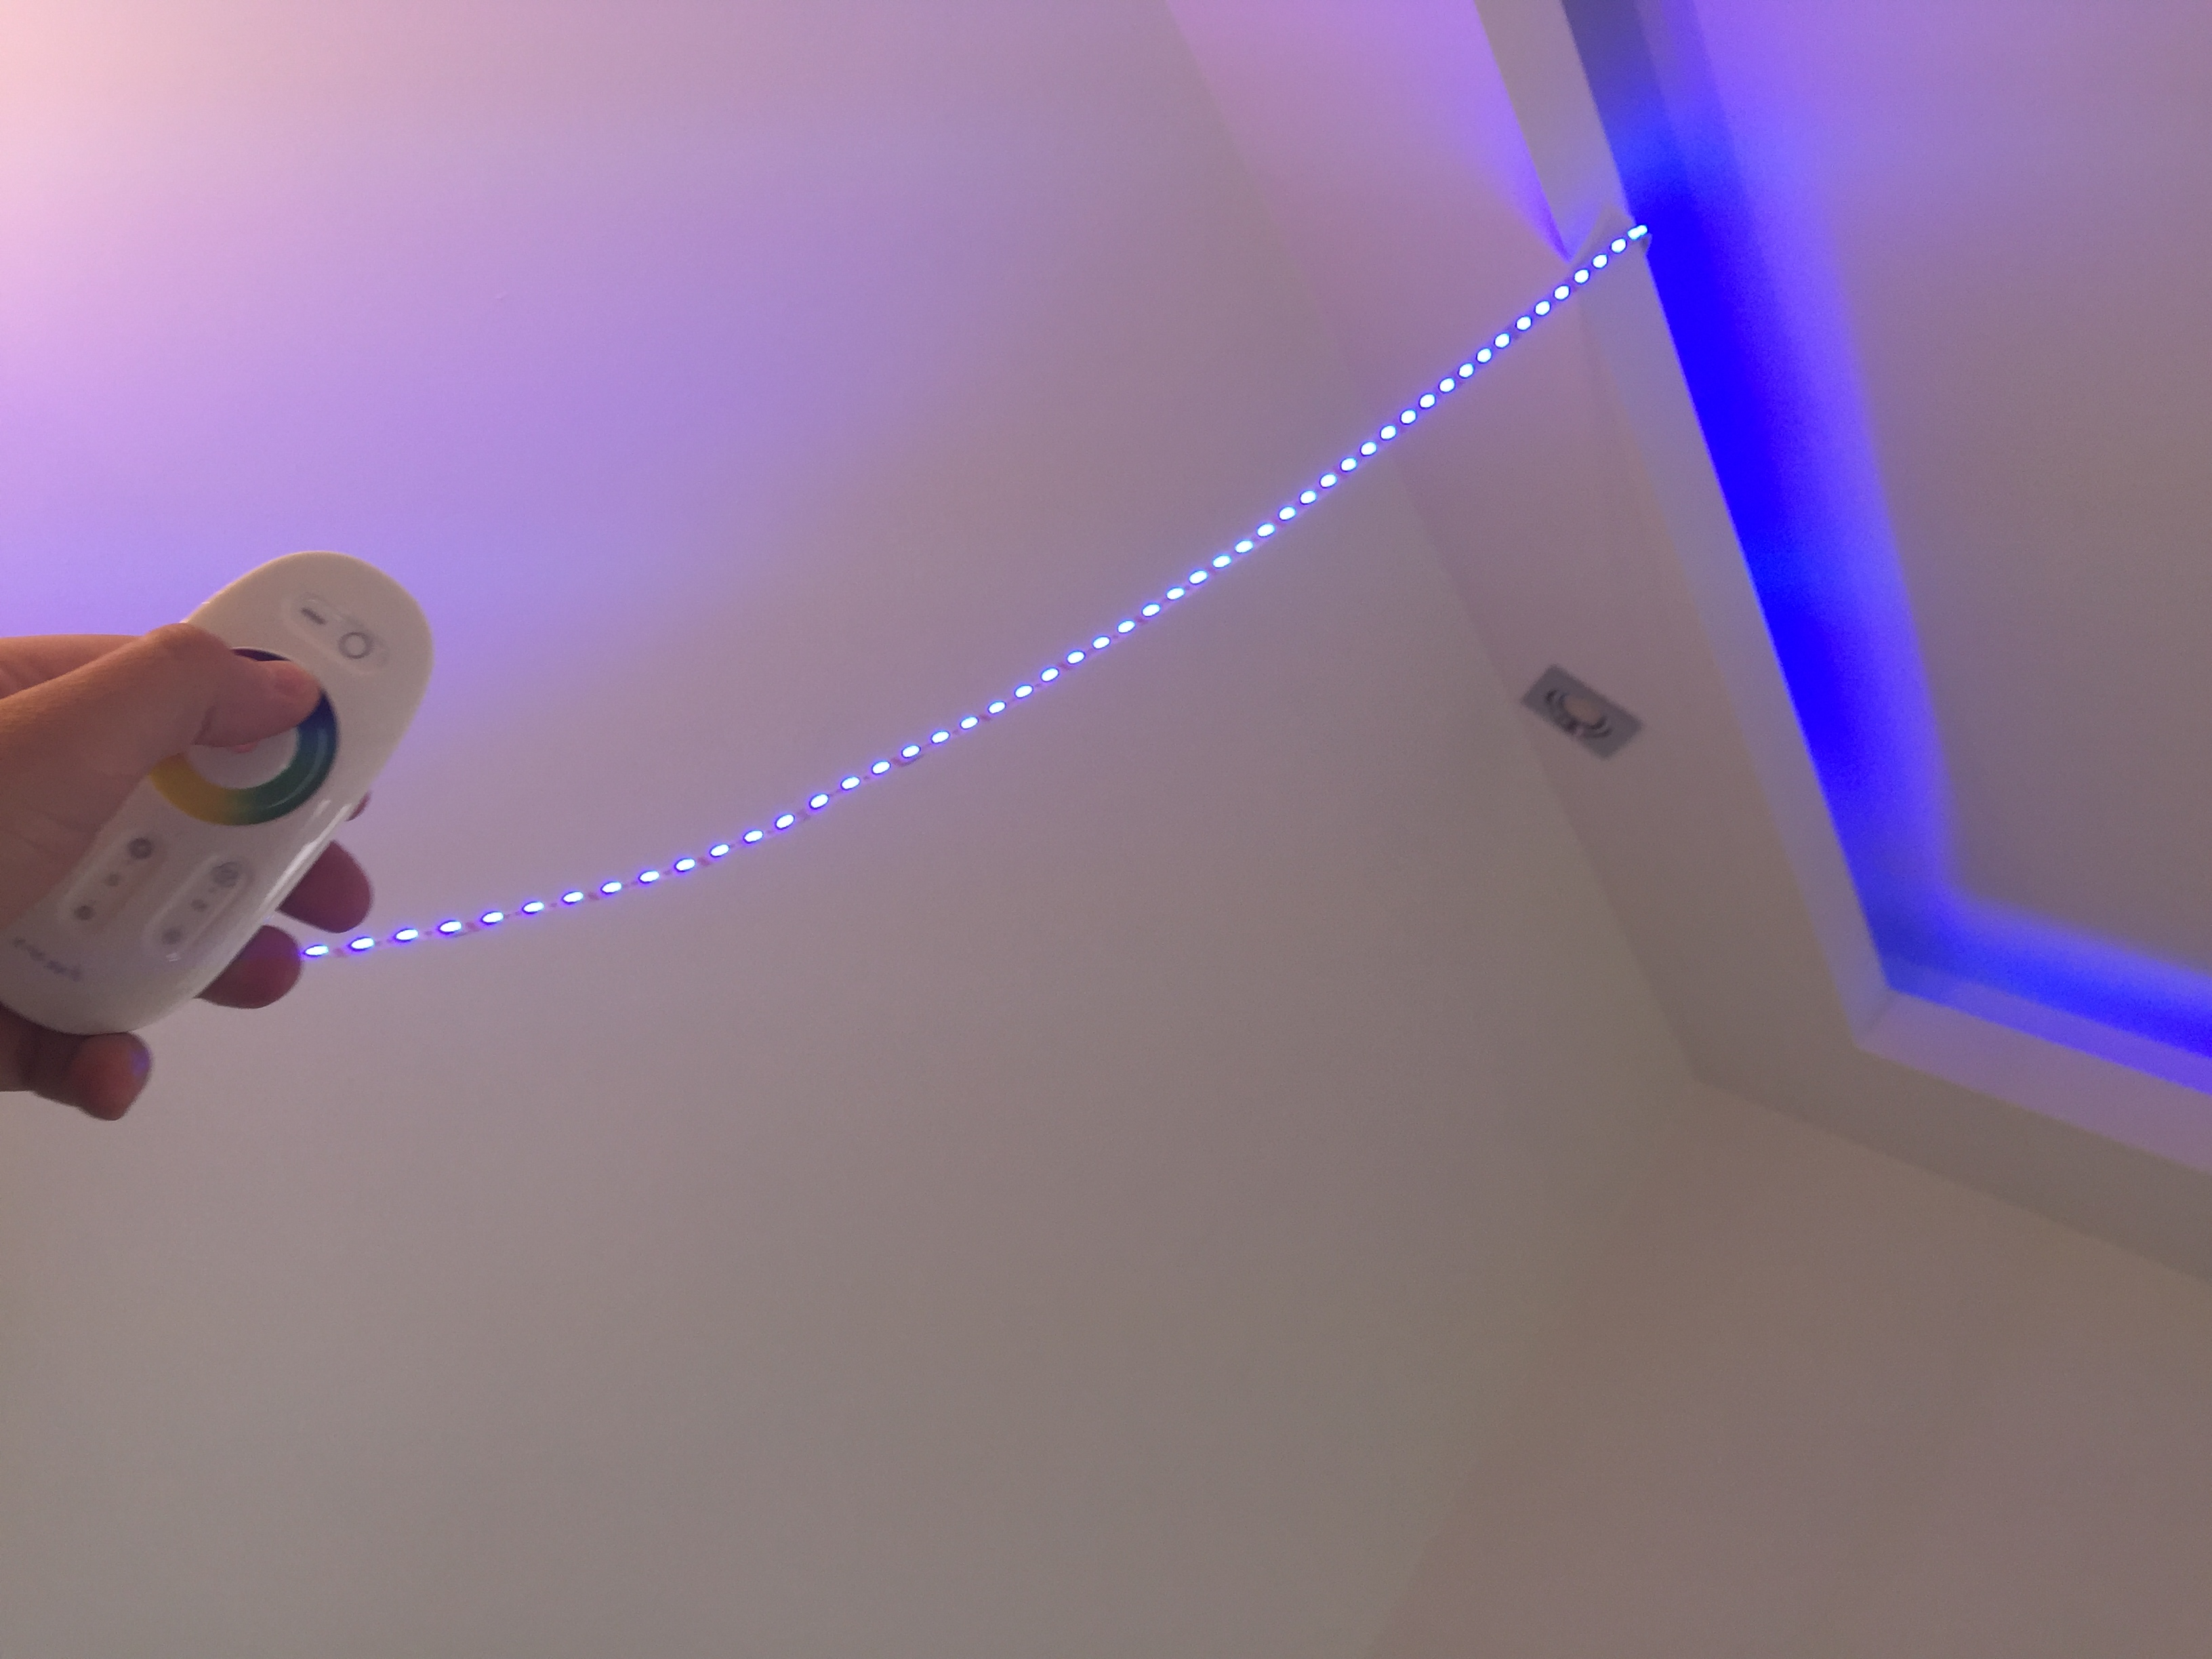
\includegraphics[width=6cm]{led3}
\caption{Oświetlenie RGB oparte o~kontroler. Przykladowy kolor 3. Opracowanie własne.}
\label{fig:led3}
\end{figure}


% zakończenie
\summary
	Nasz system monitoringu w~założeniach jest bardzo prosty. Jednak poświęciliśmy mnóstwo czasu na szukanie informacji w~internecie jak rozwiązywać kolejno napotykane problemy. Aczkolwiek takie udogodnienia niosą za sobą spore ryzyko. O~ile my naszą aplikację zabezpieczyliśmy najprostszym i~najskuteczniejszym sposobem, być może w~przyszłości będziemy chcieli prowadzić logowanie wielu użytkowników co może otworzyć lukę dla hakera. Z~drugiej strony warto korzystać z~technologii aby ułatwić sobie życie w~każdym możliwym aspekcie. 
	Uważamy, że wybrane do tej części projektu technologie idealnie sprawdzają się do naszych zastosowań. Node.js jest bardzo szybki w~porównaniu do starszych technologii i~idealnie sprawdza się w~naszym zastosowaniu.
	
	Zbudowanie od podstaw systemu inteligentnego nawadniania roślin pozwoliło nam poznać lepiej zasady działania sensorów w~rozwiązaniach Internet of Things. Utwierdziliśmy się w~przekonaniu, że rozwiązania inteligentnych przedmiotów wcale nie muszą być drogie. Nie są też trudne w~budowie. w~internecie jest dużo poradników i~materiałów na temat różnych projektów, dzięki którym bez problemu możemy zbudować podobne systemy u~siebie w~domu. 
	
	Wprowadzenie powiadomień mailowych znacznie ułatwiło nam wyhodowanie rośliny, ale po zagłębieniu się w~temat internetu rzeczy zrozumieliśmy, że nie chodzi o~to by przedmioty były tylko podłączone do sieci. Cała idea polega na tym by rzeczy zaczęły same wykonywać niektóre czynności. Dlatego w~przyszłości zamierzamy dodać funkcjonalność która sprawi, że nasz projekt stanie się prawdziwym inteligentnym systemem. Mamy w~planach dodanie silniczka - małej pompy wodnej która będzie automatycznie podlewać rośliny. Dzięki temu ograniczymy naszą aktywność, tylko do uzupełniania pojemnika z~woda. 
	
	Uważamy, że wykorzystanie Arduino pozwoliło nam na zrozumieć jak działa większość rzeczy IoT. Dowiedzieliśmy się czym tak naprawdę są inteligentne rzeczy i~w jakim kierunku rozwija się ta dziedzina. Potrafimy spojrzeć na urządzenia z~innej strony i~łatwiej jest nam zrozumieć działania tych przedmiotów.

% załączniki (opcjonalnie):
\appendix

% literatura (obowiązkowo):
\bibliographystyle{unsrt}
\bibliography{xml}

% spis tabel (jeżeli jest potrzebny):
%\listoftables

% spis rysunków (jeżeli jest potrzebny):
\listoffigures

\oswiadczenie

\end{document}